%&preformat-disser
\RequirePackage[l2tabu,orthodox]{nag} % Раскомментировав, можно в логе получать рекомендации относительно правильного использования пакетов и предупреждения об устаревших и нерекомендуемых пакетах
% Формат А4, 14pt (ГОСТ Р 7.0.11-2011, 5.3.6)
\documentclass[a4paper,14pt,oneside,openany]{memoir}

\input{common/setup}            % общие настройки шаблона
\input{common/packages}         % Пакеты общие для диссертации и автореферата
\synopsisfalse                      % Этот документ --- не автореферат
\input{Dissertation/dispackages}    % Пакеты для диссертации
\input{Dissertation/userpackages}   % Пакеты для специфических пользовательских задач

\input{Dissertation/setup}      % Упрощённые настройки шаблона

\input{common/newnames}         % Новые переменные, для всего проекта

%%% Основные сведения %%%
\newcommand{\thesisAuthorLastName}{\fixme{Дмитриев}}
\newcommand{\thesisAuthorOtherNames}{\fixme{Михаил Евгеньевич}}
\newcommand{\thesisAuthorInitials}{\fixme{М.\,Е.}}
\newcommand{\thesisAuthor}             % Диссертация, ФИО автора
{%
    \texorpdfstring{% \texorpdfstring takes two arguments and uses the first for (La)TeX and the second for pdf
        \thesisAuthorLastName~\thesisAuthorOtherNames% так будет отображаться на титульном листе или в тексте, где будет использоваться переменная
    }{%
        \thesisAuthorLastName, \thesisAuthorOtherNames% эта запись для свойств pdf-файла. В таком виде, если pdf будет обработан программами для сбора библиографических сведений, будет правильно представлена фамилия.
    }
}
\newcommand{\thesisAuthorShort}        % Диссертация, ФИО автора инициалами
{\thesisAuthorInitials~\thesisAuthorLastName}
%\newcommand{\thesisUdk}                % Диссертация, УДК
%{\fixme{xxx.xxx}}
\newcommand{\thesisTitle}              % Диссертация, название
{\fixme{Разработка интернет магазина виртуальных виделенных серверов}}
\newcommand{\thesisSpecialtyNumber}    % Диссертация, специальность, номер
{\fixme{XX.XX.XX}}
\newcommand{\thesisSpecialtyTitle}     % Диссертация, специальность, название (название взято с сайта ВАК для примера)
{\fixme{Технология обработки, хранения и~переработки злаковых, бобовых культур,
крупяных продуктов, плодоовощной продукции и~виноградарства}}
%% \newcommand{\thesisSpecialtyTwoNumber} % Диссертация, вторая специальность, номер
%% {\fixme{XX.XX.XX}}
%% \newcommand{\thesisSpecialtyTwoTitle}  % Диссертация, вторая специальность, название
%% {\fixme{Теория и~методика физического воспитания, спортивной тренировки,
%% оздоровительной и~адаптивной физической культуры}}
\newcommand{\thesisDegree}             % Диссертация, ученая степень
{\fixme{кандидата физико-математических наук}}
\newcommand{\thesisDegreeShort}        % Диссертация, ученая степень, краткая запись
{\fixme{канд. физ.-мат. наук}}
\newcommand{\thesisCity}               % Диссертация, город написания диссертации
{\fixme{Город}}
\newcommand{\thesisYear}               % Диссертация, год написания диссертации
{\fixme{20XX}}
\newcommand{\thesisOrganization}       % Диссертация, организация
{\fixme{Федеральное государственное автономное образовательное учреждение высшего
образования <<Длинное название образовательного учреждения <<АББРЕВИАТУРА>>}}
\newcommand{\thesisOrganizationShort}  % Диссертация, краткое название организации для доклада
{\fixme{НазУчДисРаб}}

\newcommand{\thesisInOrganization}     % Диссертация, организация в предложном падеже: Работа выполнена в ...
{\fixme{учреждении с~длинным длинным длинным длинным названием, в~котором
выполнялась данная диссертационная работа}}

%% \newcommand{\supervisorDead}{}           % Рисовать рамку вокруг фамилии
\newcommand{\supervisorFio}              % Научный руководитель, ФИО
{\fixme{Фамилия Имя Отчество}}
\newcommand{\supervisorRegalia}          % Научный руководитель, регалии
{\fixme{уч. степень, уч. звание}}
\newcommand{\supervisorFioShort}         % Научный руководитель, ФИО
{\fixme{И.\,О.~Фамилия}}
\newcommand{\supervisorRegaliaShort}     % Научный руководитель, регалии
{\fixme{уч.~ст.,~уч.~зв.}}

%% \newcommand{\supervisorTwoDead}{}        % Рисовать рамку вокруг фамилии
%% \newcommand{\supervisorTwoFio}           % Второй научный руководитель, ФИО
%% {\fixme{Фамилия Имя Отчество}}
%% \newcommand{\supervisorTwoRegalia}       % Второй научный руководитель, регалии
%% {\fixme{уч. степень, уч. звание}}
%% \newcommand{\supervisorTwoFioShort}      % Второй научный руководитель, ФИО
%% {\fixme{И.\,О.~Фамилия}}
%% \newcommand{\supervisorTwoRegaliaShort}  % Второй научный руководитель, регалии
%% {\fixme{уч.~ст.,~уч.~зв.}}

\newcommand{\opponentOneFio}           % Оппонент 1, ФИО
{\fixme{Фамилия Имя Отчество}}
\newcommand{\opponentOneRegalia}       % Оппонент 1, регалии
{\fixme{доктор физико-математических наук, профессор}}
\newcommand{\opponentOneJobPlace}      % Оппонент 1, место работы
{\fixme{Не очень длинное название для места работы}}
\newcommand{\opponentOneJobPost}       % Оппонент 1, должность
{\fixme{старший научный сотрудник}}

\newcommand{\opponentTwoFio}           % Оппонент 2, ФИО
{\fixme{Фамилия Имя Отчество}}
\newcommand{\opponentTwoRegalia}       % Оппонент 2, регалии
{\fixme{кандидат физико-математических наук}}
\newcommand{\opponentTwoJobPlace}      % Оппонент 2, место работы
{\fixme{Основное место работы c длинным длинным длинным длинным названием}}
\newcommand{\opponentTwoJobPost}       % Оппонент 2, должность
{\fixme{старший научный сотрудник}}

%% \newcommand{\opponentThreeFio}         % Оппонент 3, ФИО
%% {\fixme{Фамилия Имя Отчество}}
%% \newcommand{\opponentThreeRegalia}     % Оппонент 3, регалии
%% {\fixme{кандидат физико-математических наук}}
%% \newcommand{\opponentThreeJobPlace}    % Оппонент 3, место работы
%% {\fixme{Основное место работы c длинным длинным длинным длинным названием}}
%% \newcommand{\opponentThreeJobPost}     % Оппонент 3, должность
%% {\fixme{старший научный сотрудник}}

\newcommand{\leadingOrganizationTitle} % Ведущая организация, дополнительные строки. Удалить, чтобы не отображать в автореферате
{\fixme{Федеральное государственное бюджетное образовательное учреждение высшего
профессионального образования с~длинным длинным длинным длинным названием}}

\newcommand{\defenseDate}              % Защита, дата
{\fixme{DD mmmmmmmm YYYY~г.~в~XX часов}}
\newcommand{\defenseCouncilNumber}     % Защита, номер диссертационного совета
{\fixme{Д\,123.456.78}}
\newcommand{\defenseCouncilTitle}      % Защита, учреждение диссертационного совета
{\fixme{Название учреждения}}
\newcommand{\defenseCouncilAddress}    % Защита, адрес учреждение диссертационного совета
{\fixme{Адрес}}
\newcommand{\defenseCouncilPhone}      % Телефон для справок
{\fixme{+7~(0000)~00-00-00}}

\newcommand{\defenseSecretaryFio}      % Секретарь диссертационного совета, ФИО
{\fixme{Фамилия Имя Отчество}}
\newcommand{\defenseSecretaryRegalia}  % Секретарь диссертационного совета, регалии
{\fixme{д-р~физ.-мат. наук}}            % Для сокращений есть ГОСТы, например: ГОСТ Р 7.0.12-2011 + http://base.garant.ru/179724/#block_30000

\newcommand{\synopsisLibrary}          % Автореферат, название библиотеки
{\fixme{Название библиотеки}}
\newcommand{\synopsisDate}             % Автореферат, дата рассылки
{\fixme{DD mmmmmmmm YYYY года}}

% To avoid conflict with beamer class use \providecommand
\providecommand{\keywords}%            % Ключевые слова для метаданных PDF диссертации и автореферата
{}
             % Основные сведения
\input{common/fonts}            % Определение шрифтов (частичное)
\input{common/styles}           % Стили общие для диссертации и автореферата
\input{Dissertation/disstyles}  % Стили для диссертации
\input{Dissertation/userstyles} % Стили для специфических пользовательских задач

%%% Библиография. Выбор движка для реализации %%%
% Здесь только проверка установленного ключа. Сама настройка выбора движка
% размещена в common/setup.tex
\ifnumequal{\value{bibliosel}}{0}{%
    \input{biblio/predefined}   % Встроенная реализация с загрузкой файла через движок bibtex8
}{
    \input{biblio/biblatex}     % Реализация пакетом biblatex через движок biber
}

% Вывести информацию о выбранных опциях в лог сборки
\typeout{Selected options:}
\typeout{Draft mode: \arabic{draft}}
\typeout{Font: \arabic{fontfamily}}
\typeout{AltFont: \arabic{usealtfont}}
\typeout{Bibliography backend: \arabic{bibliosel}}
\typeout{Precompile images: \arabic{imgprecompile}}
% Вывести информацию о версиях используемых библиотек в лог сборки
\listfiles

%%% Управление компиляцией отдельных частей диссертации %%%
% Необходимо сначала иметь полностью скомпилированный документ, чтобы все
% промежуточные файлы были в наличии
% Затем, для вывода отдельных частей можно воспользоваться командой \includeonly
% Ниже примеры использования команды:
%
%\includeonly{Dissertation/part2}
%\includeonly{Dissertation/contents,Dissertation/appendix,Dissertation/conclusion}
%
% Если все команды закомментированы, то документ будет выведен в PDF файл полностью

\begin{document}

\input{common/renames}                 % Переопределение именований

%%% Структура диссертации (ГОСТ Р 7.0.11-2011, 4)
% \include{Dissertation/title}           % Титульный лист
% \include{Dissertation/contents}        % Оглавление
\ifnumequal{\value{contnumfig}}{1}{}{\counterwithout{figure}{chapter}}
\ifnumequal{\value{contnumtab}}{1}{}{\counterwithout{table}{chapter}}
\chapter*{Введение}                         % Заголовок
\addcontentsline{toc}{chapter}{Введение}    % Добавляем его в оглавление

\newcommand{\actuality}{}
\newcommand{\progress}{}
\newcommand{\aim}{{\textbf\aimTXT}}
\newcommand{\tasks}{\textbf{\tasksTXT}}
% \newcommand{\novelty}{\textbf{\noveltyTXT}}
% \newcommand{\influence}{\textbf{\influenceTXT}}
% \newcommand{\methods}{\textbf{\methodsTXT}}
% \newcommand{\defpositions}{\textbf{\defpositionsTXT}}
% \newcommand{\reliability}{\textbf{\reliabilityTXT}}
% \newcommand{\probation}{\textbf{\probationTXT}}
% \newcommand{\contribution}{\textbf{\contributionTXT}}
% \newcommand{\publications}{\textbf{\publicationsTXT}}

{\actuality}
Сегодня тот факт, что виртуализация является чрезвычайно актуальной и востребованной технологией, больше не вызывает сомнений. Применительно к настольным компьютерам и серверам виртуализация - это создание нескольких «виртуальных» машин на одном физическом сервере или компьютере, каждая из которых может иметь свою собственную среду - операционную систему, приложения, пользовательские настройки и т.д. . Кроме того, такие виртуальные машины ( ВМ) полностью изолированы друг от друга и ведут себя как отдельные физические компьютеры.

Виртуализация может значительно повысить эффективность оборудования, имеющегося в распоряжении предприятия, путем консолидации рабочих нагрузок на относительно небольшом количестве физических компьютеров. В свою очередь, повышение эффективности использования аппаратных ресурсов может сократить количество серверного оборудования и значительно снизить эксплуатационные расходы на поддержание ИТ-инфраструктуры предприятия.

Во-вторых, многие организации в последнее время практикуют классический подход к выделению отдельного сервера для каждой новой задачи. Так, например, один сервер отображается для СУБД, а другой - для хранилища файлов. Эта стратегия обеспечивает хорошую изоляцию несвязанных приложений, однако по мере роста предприятия экспоненциальный рост серверного парка, в результате чего вся ИТ-инфраструктура быстро становится плохо управляемой. В то же время значительное количество времени и человеческих ресурсов расходуется на обслуживание рабочих станций, устранение сбоев и простоев, а также возникают проблемы с резервным копированием, восстановлением данных и т.д. .

С помощью виртуализации можно организовать более эффективное централизованное управление вычислительными ресурсами и упростить администрирование оборудования без нарушения изоляции несвязанных приложений. Это достигается благодаря новым возможностям виртуализации для управления ресурсами, которые сложно или невозможно реализовать с использованием традиционных подходов.

Сегодня покупка серверного оборудования в большинстве случаев нецелесообразна. Это связано, прежде всего, с высокой стоимостью оборудования и необходимостью организации помещений для из размещения. Гораздо удобнее воспользоваться арендой выделенных виртуальных сервером. Такая услуга актуальна в следующих ситуациях:
\begin{itemize}
  \item Использование ресурса с огромными объемами данных или постоянно оперируемого цифрового контента, для хранения которого необходим достаточный объем дисковой памяти;
  \item Работа с сайтом, содержащим большое количество информации;
  \item Без выделенного сервера нельзя обойтись, если общий хостинг не имеет достаточного количества ресурсов, способных поддерживать стабильную работу определенного сайта;
  \item При работе с порталами, занимающимися постоянной рассылкой электронной почты в больших количествах;
  \item В ходе использования ресурсов, отличающихся высоким уровнем посещаемости.
\end{itemize}


Пользователи виртуальных выделенных серверов получают права администратора.
Последнее позволяет совершенно свободно управлять системой, настраивая ее под личные нужды, редактировать, устанавливать программы.
В этом случае все ресурсы (программы, базы данных, приложения), расположенные на выделенном сервере, будут доступны с любого компьютера, подключенного к сети, как если бы они находились в локальной сети.
Крупные компании, использующие эти услуги, смогут сэкономить на покупке лицензионного программного обеспечения, т.к., программа, установленная на виртуальном сервере, может использоваться многими компьютерами.

% {\progress}
% Этот раздел должен быть отдельным структурным элементом по
% ГОСТ, но он, как правило, включается в описание актуальности
% темы. Нужен он отдельным структурынм элемементом или нет ---
% смотрите другие диссертации вашего совета, скорее всего не нужен.

{\aim} данной работы является разработать интернет-магазин выделенных виртуальных серверов.

Для~достижения поставленной цели необходимо было решить следующие {\tasks}:
\begin{enumerate}
  \item Исследовать прикладную область и технологии этой области;
  \item Разработать сайт.
\end{enumerate}

% {\novelty}
% \begin{enumerate}
%   \item Впервые \ldots
%   \item Впервые \ldots
%   \item Было выполнено оригинальное исследование \ldots
% \end{enumerate}

% {\influence} \ldots

% {\methods} \ldots

% {\defpositions}
% \begin{enumerate}
%   \item Первое положение
%   \item Второе положение
%   \item Третье положение
%   \item Четвертое положение
% \end{enumerate}
% В папке Documents можно ознакомиться в решением совета из Томского ГУ
% в~файле \verb+Def_positions.pdf+, где обоснованно даются рекомендации
% по~формулировкам защищаемых положений.

% {\reliability} полученных результатов обеспечивается \ldots \ Результаты находятся в соответствии с результатами, полученными другими авторами.


% {\probation}
% Основные результаты работы докладывались~на:
% перечисление основных конференций, симпозиумов и~т.\:п.

% {\contribution} Автор принимал активное участие \ldots

% \ifnumequal{\value{bibliosel}}{0}
% {%%% Встроенная реализация с загрузкой файла через движок bibtex8. (При желании, внутри можно использовать обычные ссылки, наподобие `\cite{vakbib1,vakbib2}`).
%     {\publications} Основные результаты по теме диссертации изложены
%     в~XX~печатных изданиях,
%     X из которых изданы в журналах, рекомендованных ВАК,
%     X "--- в тезисах докладов.
% }%
% {%%% Реализация пакетом biblatex через движок biber
%     \begin{refsection}[bl-author]
%         % Это refsection=1.
%         % Процитированные здесь работы:
%         %  * подсчитываются, для автоматического составления фразы "Основные результаты ..."
%         %  * попадают в авторскую библиографию, при usefootcite==0 и стиле `\insertbiblioauthor` или `\insertbiblioauthorgrouped`
%         %  * нумеруются там в зависимости от порядка команд `\printbibliography` в этом разделе.
%         %  * при использовании `\insertbiblioauthorgrouped`, порядок команд `\printbibliography` в нём должен быть тем же (см. biblio/biblatex.tex)
%         %
%         % Невидимый библиографический список для подсчёта количества публикаций:
%         \printbibliography[heading=nobibheading, section=1, env=countauthorvak,          keyword=biblioauthorvak]%
%         \printbibliography[heading=nobibheading, section=1, env=countauthorwos,          keyword=biblioauthorwos]%
%         \printbibliography[heading=nobibheading, section=1, env=countauthorscopus,       keyword=biblioauthorscopus]%
%         \printbibliography[heading=nobibheading, section=1, env=countauthorconf,         keyword=biblioauthorconf]%
%         \printbibliography[heading=nobibheading, section=1, env=countauthorother,        keyword=biblioauthorother]%
%         \printbibliography[heading=nobibheading, section=1, env=countauthor,             keyword=biblioauthor]%
%         \printbibliography[heading=nobibheading, section=1, env=countauthorvakscopuswos, filter=vakscopuswos]%
%         \printbibliography[heading=nobibheading, section=1, env=countauthorscopuswos,    filter=scopuswos]%
%         %
%         \nocite{*}%
%         %
%         {\publications} Основные результаты по теме диссертации изложены в~\arabic{citeauthor}~печатных изданиях,
%         \arabic{citeauthorvak} из которых изданы в журналах, рекомендованных ВАК\sloppy%
%         \ifnum \value{citeauthorscopuswos}>0%
%             , \arabic{citeauthorscopuswos} "--- в~периодических научных журналах, индексируемых Web of~Science и Scopus\sloppy%
%         \fi%
%         \ifnum \value{citeauthorconf}>0%
%             , \arabic{citeauthorconf} "--- в~тезисах докладов.
%         \else%
%             .
%         \fi
%     \end{refsection}%
%     \begin{refsection}[bl-author]
%         % Это refsection=2.
%         % Процитированные здесь работы:
%         %  * попадают в авторскую библиографию, при usefootcite==0 и стиле `\insertbiblioauthorimportant`.
%         %  * ни на что не влияют в противном случае
%         \nocite{vakbib2}%vak
%         \nocite{bib1}%other
%         \nocite{confbib1}%conf
%     \end{refsection}%
%         %
%         % Всё, что вне этих двух refsection, это refsection=0,
%         %  * для диссертации - это нормальные ссылки, попадающие в обычную библиографию
%         %  * для автореферата:
%         %     * при usefootcite==0, ссылка корректно сработает только для источника из `external.bib`. Для своих работ --- напечатает "[0]" (и даже Warning не вылезет).
%         %     * при usefootcite==1, ссылка сработает нормально. В авторской библиографии будут только процитированные в refsection=0 работы.
%         %
%         % Невидимый библиографический список для подсчёта количества внешних публикаций
%         % Используется, чтобы убрать приставку "А" у работ автора, если в автореферате нет
%         % цитирований внешних источников.
%         % Замедляет компиляцию
%     \ifsynopsis
%     \ifnumequal{\value{draft}}{0}{
%       \printbibliography[heading=nobibheading, section=0, env=countexternal,          keyword=biblioexternal]%
%     }{}
%     \fi
% }

% При использовании пакета \verb!biblatex! будут подсчитаны все работы, добавленные
% в файл \verb!biblio/author.bib!. Для правильного подсчёта работ в~различных
% системах цитирования требуется использовать поля:
% \begin{itemize}
%         \item \texttt{authorvak} если публикация индексирована ВАК,
%         \item \texttt{authorscopus} если публикация индексирована Scopus,
%         \item \texttt{authorwos} если публикация индексирована Web of Science,
%         \item \texttt{authorconf} для докладов конференций,
%         \item \texttt{authorother} для других публикаций.
% \end{itemize}
% Для подсчёта используются счётчики:
% \begin{itemize}
%         \item \texttt{citeauthorvak} для работ, индексируемых ВАК,
%         \item \texttt{citeauthorscopus} для работ, индексируемых Scopus,
%         \item \texttt{citeauthorwos} для работ, индексируемых Web of Science,
%         \item \texttt{citeauthorvakscopuswos} для работ, индексируемых одной из трёх баз,
%         \item \texttt{citeauthorscopuswos} для работ, индексируемых Scopus или Web of~Science,
%         \item \texttt{citeauthorconf} для докладов на конференциях,
%         \item \texttt{citeauthorother} для остальных работ,
%         \item \texttt{citeauthor} для суммарного количества работ.
% \end{itemize}
% % Счётчик \texttt{citeexternal} используется для подсчёта процитированных публикаций.

% Для добавления в список публикаций автора работ, которые не были процитированы в
% автореферате требуется их~перечислить с использованием команды \verb!\nocite! в
% \verb!Synopsis/content.tex!.
 % Характеристика работы по структуре во введении и в автореферате не отличается (ГОСТ Р 7.0.11, пункты 5.3.1 и 9.2.1), потому её загружаем из одного и того же внешнего файла, предварительно задав форму выделения некоторым параметрам

%% на случай ошибок оставляю исходный кусок на месте, закомментированным
%Полный объём диссертации составляет  \ref*{TotPages}~страницу
%с~\totalfigures{}~рисунками и~\totaltables{}~таблицами. Список литературы
%содержит \total{citenum}~наименований.
%
% Полный объём диссертации составляет
% \formbytotal{TotPages}{страниц}{у}{ы}{}, включая
% \formbytotal{totalcount@figure}{рисун}{ок}{ка}{ков} и
% \formbytotal{totalcount@table}{таблиц}{у}{ы}{}.   Список литературы содержит
% \formbytotal{citenum}{наименован}{ие}{ия}{ий}.
    % Введение
% \ifnumequal{\value{contnumfig}}{1}{\counterwithout{figure}{chapter}
% }{\counterwithin{figure}{chapter}}
% \ifnumequal{\value{contnumtab}}{1}{\counterwithout{table}{chapter}
% }{\counterwithin{table}{chapter}}
\chapter{Описание прикладной области}\label{ch:ch1}
\section{Интернет-хостинг}\label{sec:ch1/sec1}
Интернет-хостинг - это служба, которая предоставляет интернет-серверы, позволяя организациям и частным лицам размещать контент в Интернет. Существуют различные уровни обслуживания и различные виды предлагаемых услуг.

Распространенным видом хостинга является веб-хостинг. Большинство хостинг-провайдеров предлагают комбинацию услуг, например, хостинг электронной почты.

Чаще всего интернет-хостинг предоставляет сервер с хорошей пропуской способностью интернет соединения, на котором клиенты могут запускать любые приложения.

\subsection{Dedicated Server. Выделенный сервер.}\label{sec:ds_hosting}
Выделенный хостинг - это вариант хостинга в Интернете, в котором физический сервер (или серверы) выделяются для одного бизнес-клиента. Заказчик имеет полный контроль над машиной, поэтому он может оптимизировать ее для своих уникальных требований, включая производительность и безопасность. Хостинг-провайдер предоставляет физический сервер и среду, сопутствующие услуги и техническую поддержку.

\subsection{VPS. Виртуальный выделенный сервер}\label{sec:vps_hosting}
VPS - это сокращение от Virtual Private Server (Виртуальный выделенный сервер). VPS хостинг - одна из самых популярных услуг хостинга, которую можно выбрать для размещения сайта и приложений. Для работы используется технология виртуализации, позволяющая предоставить выделенные (частные) ресурсы на сервере с несколькими пользователями.

Это более безопасное и стабильное решение, чем виртуальный хостинг, где клиент не получает выделенного серверного пространства. Тем не менее, VPS меньше и дешевле, чем аренда всего сервера.

Хостинг VPS обычно выбирают владельцы веб-сайтов, у которых трафик среднего уровня превышает лимиты планов общего хостинга, но при этом ему не нужны ресурсы выделенного сервера, или энтузиасты, которые ипользуются выделенные сервера для своих приложений.

\subsection{Колокация}\label{sec:colo_hosting}
Колокация - услуга, состоящая в том, что клиенту предоставляется оборудование на своей территории (датацентре). В случаях, если оборудование тоже арендуется клиентом, это называется "арендой выделенного сервера".

Такое размещение позволяет сэкономить на организации связи. Чаще всего колокацию используются для веб-сайтов и другим сетевым службам с большим объемом трафика, а также оборудование, к которму необходимое  доступ из многих точкек, например, VPN-концентраторы, шлюзы IP-телефонии.

\subsection{Облачный хостинг}\label{sec:cloud_hosting}
Облачный хостинг - это тип веб-хостинга, который использует несколько разных серверов для балансировки нагрузки и максимизации времени безотказной работы. Вместо использования одного сервера веб-сайт может подключиться к «кластеру», который использует ресурсы из централизованного пула. Это означает, что даже если один сервер выходит из строя, другой начинает работать, что повышает отказоуствойчивость системы.

Визуализируйте облако можно представить сеть взаимосвязанных компьютеров. Чем больше компьютеров подключено в сети, тем больше ресурсов добавляется в общее облако.

С облачным хостингом клиент получает часть так называемого облачного кластера. В отличие от традиционного веб-хостинга, где клиент получает определенное количество места с одного сервера.

Основные преимущества облачного хостинга заключаются во времени безотказной работы, изолированности ресурсов, простоте масштабирования и выделенных внешних адресах.

\section{Виртуализация}\label{sec:ch1/sec2}
\subsection{Описание}\label{sec:virt_decs}
Виртуализация использует программное обеспечение для создания уровня абстракции над компьютерным оборудованием, которое позволяет разделить аппаратные элементы одного компьютера - процессоры, память, хранилище и т.д. - на несколько виртуальных компьютеров, обычно называемых виртуальными машинами (ВМ). Каждая виртуальная машина работает со своей собственной операционной системой (ОС) и ведет себя как независимый компьютер, даже если она работает только на части фактического компьютерного оборудования.

Из этого следует, что виртуализация позволяет более эффективно использовать физическое компьютерное оборудование и обеспечивает большую отдачу от вложений в оборудование организации.

Сегодня виртуализация является стандартной практикой в корпоративной ИТ-архитектуре. Это также технология, которая управляет экономикой облачных вычислений. Виртуализация позволяет пользователям облачных вычислений приобретать только те вычислительные ресурсы, которые им необходимы, когда им они необходимо, и экономически эффективно масштабировать эти ресурсы по мере роста их рабочих нагрузок.

\subsection{Объекты виртуализации}\label{sec:virt_objs}
\textbf{Операционные системы.} 
Виртуализация операционных систем — это метод размещения множества «гостевых» операционных систем (guest) поверх одной операционной системы-«хозяина» (host). Изолированные образы ОС называют «контейнерами», «виртуальными частными серверами» (Virtual Private Server, VPS) или «виртуальными средами» (Virtual Environment,VE). С точки зрения хоста VPS или VE выглядит как настоящий сервер. Этот тип виртуализации реализован во многих операционных системах: IBM AIX (технология WPARs), HP-UX (HP vPars), Sun Solaris (Container/Zone), FreeBSD(FreeBSD Jail), Linux (Linux-VServer, OpenVZ, Virtuozzo Containers), Windows (Virtuozzo Containers).

\textbf{Приложения.}
Виртуализация приложений преследует своей целью отделить приложения от операционной системы, сделать их мобильными и предоставить возможность для выполнения приложений в различных средах, например, на клиентском рабочем месте. Сравним: в обычной среде приложения инсталлируются непосредственно в операционную систему. Поскольку они используют общие системные ресурсы, то между ними есть вероятность возникновения конфликтов, что может приводить к нестабильности в работе ОС и даже к ее аварийному завершению. Эти негативные проявления полностью исключены, если каждое из приложений работает в защитной среде-оболочке.

\textbf{Оперативная память.}
Виртуализация оперативной памяти является обязательным условием виртуализации любого компьютера, поскольку позволяет динамически распределять память между виртуальными машинами, работающими на одной системе, под управлением одного монитора. Она устанавливает соответствие между виртуальными адресами, которые используют гостевые ОС и физическими адресами памяти машины. Аналогичную роль играет виртуализация периферийных устройств и ввода/вывода.

\textbf{Системы хранения.}
Виртуализация систем хранения — отдельная тема, она известна давно и хорошо. В нашем журнале было опубликовано несколько обзорных статей по этой проблеме.

\textbf{Данные.}
Для виртуализации данных существуют иные названия — Information-as-a-Service и Data-as-a-Service.

\textbf{Рабочие места.}
Известно множество самых разнообразных способов виртуализации, предназначенных для виртуализации рабочих мест, среди них наибольшее распространение получили несколько основных. Во-первых, удаленный доступ по сети (Single Remote Desktop) с использованием технологий PCAnywhere, Windows Remote Desktop и других. Во-вторых, Shared Desktops, модель, при которой мощный сервер с использованием технологий Citrix, Ericom Software или Terminal Services превращается в среду, на которой можно выполнять сотни и больше терминальных сессий. В-третьих, рабочему месту может быть поставлена в соответствие «виртуальная машина» (Virtual Machine Desktop). 

\subsection{Полная эмуляция}\label{sec:full_amu}
Данный вид виртуализации полностью симулирует всё аппаратное обеспечение при сохранении гостевой операционной системы в неизменном виде. При таком типе виртуализации имеется возможность запускать различные аппаратные архитектуры. Нетрудно догадаться, что данный тип эмуляции существенно нагружает вычислительные ресурсы хостовой системы, что делает работу с ней очень медленной, поэтому, данная техника используется в основном для разработки системного программного обеспечения, а также образовательных целей.

Примеры продуктов для создания эмуляторов: Bochs, PearPC, QEMU (без ускорения), Hercules Emulator.

\subsection{Частичная эмуляция (нативная виртуализация)}\label{sec:part_emu}
В этом случае виртуальная машина эмулирует лишь необходимое количество аппаратного обеспечения, чтобы она могла быть запущена изолированно. Естесственно, что подход позволяет запускать гостевые операционные системы, разработанные только для той же архитектуры, что и у хоста. Этот вид виртуализации положительно влияет на быстродействие гостевых систем по сравнению с полной эмуляцией и широко используется в настоящее время. Для увеличения быстродействия также используется следующий подход, применяется специальная «прослойка» между гостевой операционной системой и оборудованием (гипервизор), позволяющая гостевой системе напрямую обращаться к ресурсам аппаратного обеспечения. Гипервизор, называемый также «Монитор виртуальных машин» (Virtual Machine Monitor) - одно из основных понятий в мире виртуализации. Применение гипервизора существенно увеличивает быстродействие платформы, приближая его к быстродействию физической платформы. Самым большим минусом данного вида виртуализации можно отнести зависимость виртуальных машин от архитектуры аппаратной платформы.

Примеры продуктов для нативной виртуализации: VMware Workstation, VMware Server, VMware ESX Server, Virtual Iron, Virtual PC, VirtualBox, Parallels Desktop и другие.

\subsection{Виртуализация адресного пространства}\label{sec:virt_space_emu}
В данном случае, виртуальная машина симулирует несколько экземпляров аппаратного окружения. Притаком подходе имеется возможность совместно использовать ресурсы и изолировать процессы, но не позволяет разделять экземпляры гостевых операционных систем. В данном виде виртуальные машину не создаются полностью, а происходит изоляция каких-либо процессов на уровне операционной системы. В данный момент многие из известных операционных систем используют такой подход.

\subsection{Паравиртуализация}\label{sec:paravirt}
При применении паравиртуализации нет необходимости симулировать аппаратное обеспечение, используется специальный программный интерфейс (API) для взаимодействия с гостевой операционной системой. При данном подходе требуется модифицированное гостевое ядро системы. Так как при построение данного вида виртуализированного окружения необходимо модифицировать код ядра операционной системы, повсеместное внедрение данного типа не получило широкого распространения по понятным причинам.

\subsection{Виртуализация уровня операционной системы}\label{sec:os_level_virt}
Сутью данного вида виртуализации является виртуализация физического сервера на уровне операционной системы в целях создания нескольких защищенных виртуализованных серверов на одном физическом. Гостевая система, в данном случае, разделяет использование одного ядра хостовой операционной системы с другими гостевыми системами. Виртуальная машина представляет собой окружение для приложений, запускаемых изолированно. Данный тип виртуализации применяется при организации систем хостинга, когда в рамках одного экземпляра ядра требуется поддерживать несколько виртуальных серверов клиентов.

Примеры виртуализации уровня ОС: Linux-VServer, Virtuozzo, OpenVZ, Solaris Containers и FreeBSD Jails.

\subsection{Виртуализация уровня приложений}\label{sec:app_level_virt}
Данный вид виртуализации не похож на все остальные: в отличии от других способов само приложение помещается в контейнер с необходимыми элементами для своей работы: файлами реестра, конфигурационными файлами, пользовательскими и системными объектами. В результате получается приложение, не требующее установки на аналогичной платформе. При переносе такого приложения на другую машину и его запуске, виртуальное окружение, созданное для программы, разрешает конфликты между ней и операционной системой, а также другими приложениями. Такой способ виртуализации похож на поведение интерпретаторов различных языков программирования (недаром интерпретатор, Виртуальная Машина Java (JVM), тоже попадает в эту категорию).

Примером такого подхода служат: Thinstall, Altiris, Trigence, Softricity. 

\section{Обзор существующих решений}\label{sec:ch1/sec3}
\subsection{Amazon VPS}\label{sec:amazon}
Amazon Virtual Private Cloud (Amazon VPC) – это логически изолированный раздел облака Amazon Web Services (AWS), в котором можно запускать ресурсы AWS в самостоятельно заданной виртуальной сети. Таким образом можно полностью контролировать среду виртуальной сети, в том числе выбирать собственный диапазон IP‑адресов, создавать подсети, а также настраивать таблицы маршрутизации и сетевые шлюзы. Для обеспечения удобного и безопасного доступа к ресурсам и приложениям в VPC можно использовать как протокол IPv4, так и протокол IPv6.
\newline
Amazon VPS предлагает огромное количество тарифов и конфигураций, в таблице~\ref{tab:awazon_vps} описаны некоторые из них.

\begin{table} [htbp]%
  \centering
  \begin{threeparttable}% выравнивание подписи по границам таблицы
    \caption{Список некоторых тарифов ВМ Amazon VPS}
    \label{tab:awazon_vps}% label всегда желательно идти после caption
    \renewcommand{\arraystretch}{1}%% Увеличение расстояния между рядами, для улучшения восприятия.
    \begin{SingleSpace}
      \begin{tabular}{@{}@{\extracolsep{20pt}}llll@{}}
        % Вертикальные полосы не используются принципиально, как и лишние горизонтальные (допускается по ГОСТ 2.105 пункт 4.4.5) % @{} позволяет прижиматься к краям
        \toprule     %%% верхняя линейка
          Название & Вирт.ЦПУ & Память ГиБ & Цена за час \\
        \midrule %%% тонкий разделитель. Отделяет названия столбцов. Обязателен по ГОСТ 2.105 пункт 4.4.5
          a1.medium & 1 & 2 & 0,0291 USD \\
          a1.large & 2 & 4 & 0,0582 USD \\
          a1.xlarge & 4 & 8 & 0,1164 USD \\
          a1.2xlarge & 8 & 16 & 0,2328 USD \\
          a1.2xlarge & 8 & 16 & 0,2328 USD \\
          a1.4xlarge & 16 & 32 & 0,4656 USD \\
          a1.metal & 16 & 32 & 0,466 USD \\
          t3.nano & 2 & 0,5 & 0,006 USD \\
          t3.micro & 2 & 1 & 0,012 USD \\
          t3.small & 2 & 2 & 0,024 USD \\
          t3.large & 2 & 8 & 0,096 USD \\
        \bottomrule %%% нижняя линейка
      \end{tabular}%
    \end{SingleSpace}
  \end{threeparttable}
\end{table}

\subsection{Hostwinds}\label{sec:hostwinds}
Компания прдоставляет большой спект услуг - веб-хостинг, облачные вычисления, выделенные физические и виртуальные сервера, как с linux, так и с windows. Основана в 2010 году, сервера находятся в Сиэтле, Далласе и Амстердаме. 
\newline
В таблице~\ref{tab:hostwinds_vps} описаны некоторые конфигурации.

\begin{table} [htbp]%
  \centering
  \begin{threeparttable}% выравнивание подписи по границам таблицы
    \caption{Список некоторых тарифов ВМ Hostwinds}
    \label{tab:hostwinds_vps}% label всегда желательно идти после caption
    \renewcommand{\arraystretch}{1}%% Увеличение расстояния между рядами, для улучшения восприятия
    \begin{SingleSpace}
      \begin{tabular}{@{}@{\extracolsep{10pt}}lllll@{}}
        % Вертикальные полосы не используются принципиально, как и лишние горизонтальные (допускается по ГОСТ 2.105 пункт 4.4.5) % @{} позволяет прижиматься к краям
        \toprule     %%% верхняя линейка
          Вирт.ЦПУ & Память ГиБ & Хранилище ГиБ & Трафик ТБ & Цена за месяц \\
        \midrule %%% тонкий разделитель. Отделяет названия столбцов. Обязателен по ГОСТ 2.105 пункт 4.4.5
          1 & 1 & 30 & 1 & 4,49 USD \\
          1 & 2 & 50 & 2 & 8,99 USD \\
          2 & 4 & 75 & 2 & 17,09 USD \\
          2 & 6 & 100 & 2 & 26,09 USD \\
          4 & 8 & 150 & 3 & 36,09 USD \\
        \bottomrule %%% нижняя линейка
      \end{tabular}%
    \end{SingleSpace}
  \end{threeparttable}
\end{table}

\subsection{Ionos}\label{sec:ionos}
IONOS является веб-хостингом и провайдеров облаков для малого и среднего бизнеса. Компания являемся экспертами в области IaaS и предлагает портфель решений для цифрового пространства. 
Компания предоставляет большое количество услуг - регистрация доменов, конструктор сайтов, хостинг сайтов, выделенных и виртуальных серверов, облачных хранилищ.
\newline

В таблице~\ref{tab:ionos_vps} описаны некоторые конфигурации.
\begin{table} [htbp]%
  \centering
  \begin{threeparttable}% выравнивание подписи по границам таблицы
    \caption{Список некоторых тарифов ВМ Ionos}
    \label{tab:ionos_vps}% label всегда желательно идти после caption
    \renewcommand{\arraystretch}{1}%% Увеличение расстояния между рядами, для улучшения восприятия
      \begin{tabular}{@{}@{\extracolsep{10pt}}lllll@{}}
        % Вертикальные полосы не используются принципиально, как и лишние горизонтальные (допускается по ГОСТ 2.105 пункт 4.4.5) % @{} позволяет прижиматься к краям
        \toprule     %%% верхняя линейка
          Название & Вирт.ЦПУ & Память ГиБ & Хранилище ГиБ & Цена за месяц \\
        \midrule %%% тонкий разделитель. Отделяет названия столбцов. Обязателен по ГОСТ 2.105 пункт 4.4.5
          VPS S & 1 & 0,5 & 10 & 2 USD \\
          VPS M & 2 & 2 & 80 & 10 USD \\
          VPS L & 2 & 4 & 120 & 20 USD \\
          VPS XL & 4 & 8 & 160 & 30 USD \\
          VPS XXL & 6 & 12 & 240 & 30 USD \\
        \bottomrule %%% нижняя линейка
      \end{tabular}%
  \end{threeparttable}
\end{table}

\subsection{Alibabacloud}\label{sec:alibabacloud}
Компания Alibaba Cloud была основана в сентябре 2009 года. Она разрабатывает платформы для облачных вычислений и управления данными и предоставляет полный набор услуг в сфере облачных вычислений для поддержки предприятий во всем мире. Является подразделением крупнейшей китайской интернет-компании Alibaba Group. К маю 2018 году у Alibaba Cloud насчитывается несколько партнеров в России.
Услуги предоставляемые компание относятся к областям облачных вычислений, облачных хранилищ, аналитики, искуственного интеллекта, интернета вещей и платформ для разработчиков.
\newline

В таблице~\ref{tab:alibabacloud_vps} описаны некоторые конфигурации.
\begin{table} [htbp]%
  \centering
  \begin{threeparttable}% выравнивание подписи по границам таблицы
    \caption{Список некоторых тарифов ВМ Alibabacloud}
    \label{tab:alibabacloud_vps}% label всегда желательно идти после caption
    \renewcommand{\arraystretch}{1}%% Увеличение расстояния между рядами, для улучшения восприятия
    \begin{SingleSpace}
      \begin{tabular}{@{}@{\extracolsep{10pt}}lllll@{}}
        % Вертикальные полосы не используются принципиально, как и лишние горизонтальные (допускается по ГОСТ 2.105 пункт 4.4.5) % @{} позволяет прижиматься к краям
        \toprule     %%% верхняя линейка
          Вирт.ЦПУ & Память ГиБ & Хранилище ГиБ & Трафик ТБ & Цена за месяц \\
        \midrule %%% тонкий разделитель. Отделяет названия столбцов. Обязателен по ГОСТ 2.105 пункт 4.4.5
          1 & 0,5 & 20 & 1 & 3,3 USD \\
          1 & 1 & 25 & 2 & 4,5 USD \\
          1 & 2 & 50 & 3 & 9,0 USD \\
          2 & 2 & 60 & 3 & 13,5 USD \\
          2 & 4 & 80 & 4 & 18,0 USD \\
          2 & 8 & 80 & 5 & 36,0 USD \\
          4 & 16 & 320 & 6 & 72,0 USD \\
          8 & 32 & 500 & 7 & 144,0 USD \\
        \bottomrule %%% нижняя линейка
      \end{tabular}%
    \end{SingleSpace}
  \end{threeparttable}
\end{table}

\subsection{Hetzner}\label{sec:hetzner}
TODO           % Глава 1
% \chapter{Постановка требований и функциональности проекта}\label{ch:ch2}
% \section{Описание бизнес-ролей}\label{sec:ch2/sec1}


\section{Функциональные требования}\label{sec:ch2/sec2}
% \subsection{Основные требования}\label{sec:usecase_umls}

\subsection{Панель оператора}\label{sec:operator_control}
Панель оператора должна позволять пользователю с определёнными правами оператора производить действия связанные с управлением заказов, формированием отчётов и управлением списка конфигураций. Так же оператор должен иметь возможность работать со списком пользователей их аккаунтов и заказов и иметь возможность следить за выставляемыми клиентам счетами.

Для реализации необходимы страницы:
\begin{itemize}
  \item со списком клиентов;
  \item расширенной страницы клиента для оператора;
  \item оформления отчётов;
  \item редактирования списка конфигураций;
  \item списка выставленных счетов.
\end{itemize}

\subsection{Управление пользователями}\label{sec:users_control}
Для разделения прав пользователей должна быть реализована система разделения возможностей пользователей на основаниих их ролей.

Пользователь должен принадлежать одной определённой роли, что должно позволить системы быть проще, чем если бы была необходима более сложная система разделения прав на основании ролей. 

На таблице ~\ref{tab:roles} указаны основные типа ролей.
\begin{table} [htbp]% Пример записи таблицы с номером, но без отображаемого наименования
  \centering
  \begin{threeparttable}% выравнивание подписи по границам таблицы
    \caption{Список ролей пользователей}%
    \label{tab:roles}%
    \setlength\extrarowheight{4pt} %вот этим управляем расстоянием между рядами, \arraystretch даёт неудачный результат
    \setlength{\tymin}{1.9cm}% минимальная ширина столбца
    \begin{SingleSpace}
      \begin{tabulary}{\textwidth}{|@{}| >{\zz}C | >{\zz}C @{} |}
        \hline
        Роль & Описание \\ \hline
        Клиент & Пользователь имеет возможность оформлять заказы и работать с ним в рамках ограниченных операций.  \\ \hline
        Оператор & Ползователь имеет возможность управлять заказами клиентов в случае возникновения вопросов или у проблем у клиентов, запрашивать отчёты и выставлять счета. \\ \hline
      \end{tabulary}%
    \end{SingleSpace}
  \end{threeparttable}
\end{table}

\subsection{Управление заказами ВМ}\label{sec:order_control}
У клиентов должна быть возможность создавать и выполнять минимальный список операции по управлению ВМ заказа поддерживаемый системой виртуализации.
Для ВМ должно быть реализовано хранение списка состояний. 

Клиент должен иметь возможность:
\begin{itemize}
  \item запустить ВМ;
  \item выключить ВМ;
  \item перезагрузить ВМ;
  \item пересоздать ВМ.
\end{itemize}

Для реализации необходимы страницы:
\begin{itemize}
  \item выбора конфигурацией заказа (вм);
  \item подтверждения выбора и непосредственного оформления заказа; 
  \item списка заказов пользователя;
  \item страница управления заказом.
\end{itemize}

На странице заказа ВМ должна быть описана конфигурация вм и её состояние.


Для упрощения системы и её эксплуатация не должно быть возможности сменить конфигурацию ВМ. 

\subsection{Тарификация заказов}\label{sec:order_tarif}

Тарификация заказов должна проводиться по тарифам конфигураций ВМ. Конфигурация может иметь несколько тарифов с разными ценами для разных тарифицируемых периодов. 


Периоды тарификации
\begin{itemize}
  \item 1 месяц;
  \item 3 месяца; 
  \item 6 месяцев;
  \item 12 месяцев.
\end{itemize}

\subsection{Требованяи к оплате}\label{sec:order_pay}
Система должна хранить только данных о тарифах и платах (чеках) клиентов, вся оплата должна происходить через интеграцию со сторонней системой.


В своём профиле клиент должен иметь возможность увидеть список своих платежей и их статус.


При создании платежа необходимо создавать снапшот заказа и его тарифа.

\subsection{Формирование отчётов}\label{sec:report_gen}
Должна быть реализована возможность формирования определённого ряда отчётов с определёнными фильтрами.

На таблице ~\ref{tab:filters} указаны обязательные фильтры.
\begin{table} [htbp]% Пример записи таблицы с номером, но без отображаемого наименования
  \centering
  \begin{threeparttable}% выравнивание подписи по границам таблицы
    \caption{Список фильтров для формирования отчёта}%
    \label{tab:filters}%
    \setlength\extrarowheight{4pt} %вот этим управляем расстоянием между рядами, \arraystretch даёт неудачный результат
    \setlength{\tymin}{1.9cm}% минимальная ширина столбца
    \begin{SingleSpace}
      \begin{tabulary}{\textwidth}{|@{}| >{\zz}C | >{\zz}C @{} |}
        \hline
        Фильтр & Описание \\ \hline
        Тип отчёта &  Выбор типа из списка\\ \hline
        Диапазон дат & Выбор диапазона дат в форме календаря \\ \hline
      \end{tabulary}%
    \end{SingleSpace}
  \end{threeparttable}
\end{table}

В системе должна быть возможность указывать типы полей значений и алгоритмы вычисления для них для обеспечения упрощения создания новых типов отчётов и специальных полей в них.


Отчёт должен формироваться в формате CSV и отправляться на электронную почту запрасившего его оператора. Стобцы отчёта должны быть определены на этапе разработки.

\section{Нефункциональные требования}\label{sec:ch2/sec3}
Система должна обладать следующими качествами:
\begin{itemize}
  \item используется язык Ruby
  \item используется фреймворк Ruby on Rails
  \item используется СУБД PostgreSQL
  \item используется Sidekiq для фоновых задач
  \item система разрабатывается для ОС семейства *nix
  \item используется сервер unicorn
  \item используется nginx в роли реверс-прокси
  \item используется система виртуализации OpenStack
  \item оплата производится через систему Яндекс.Касса
\end{itemize}

\section{Диаграммы прецедентов}\label{sec:ch2/sec4}
На рисунке~\ref{fig:umls_register_ucesace} показан сценарий регистрации нового клиента.
\begin{figure}[ht]
  \centerfloat{
    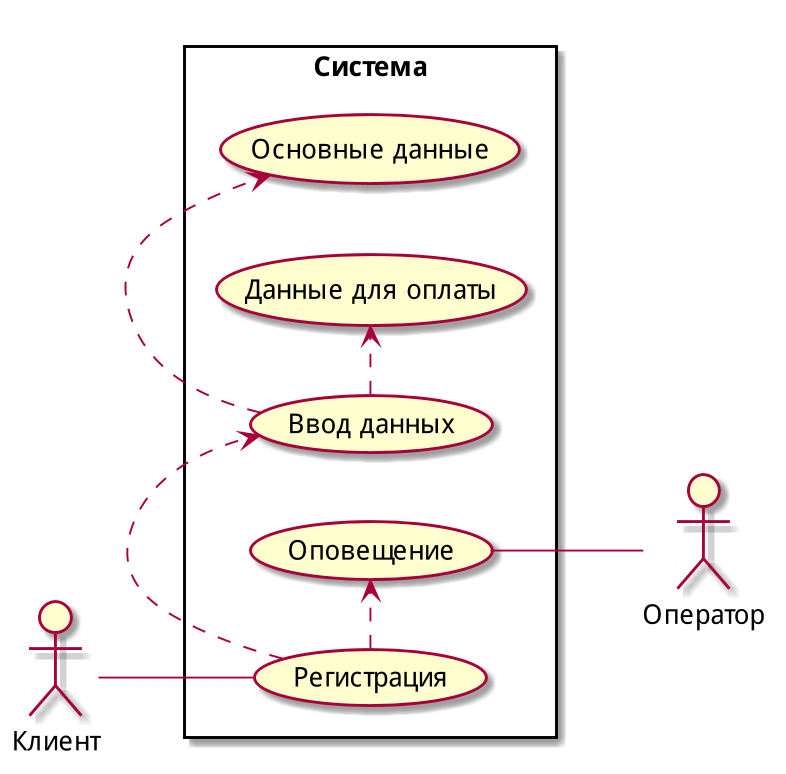
\includegraphics[scale=0.27]{umls/register_ucesace}
  }
  \caption{Сценарий регистрации клиента.}\label{fig:umls_register_ucesace}
\end{figure}

На рисунке~\ref{fig:umls_make_order_usecase} показан сценарий оформления заказа клиентом.
\begin{figure}[ht]
  \centerfloat{
    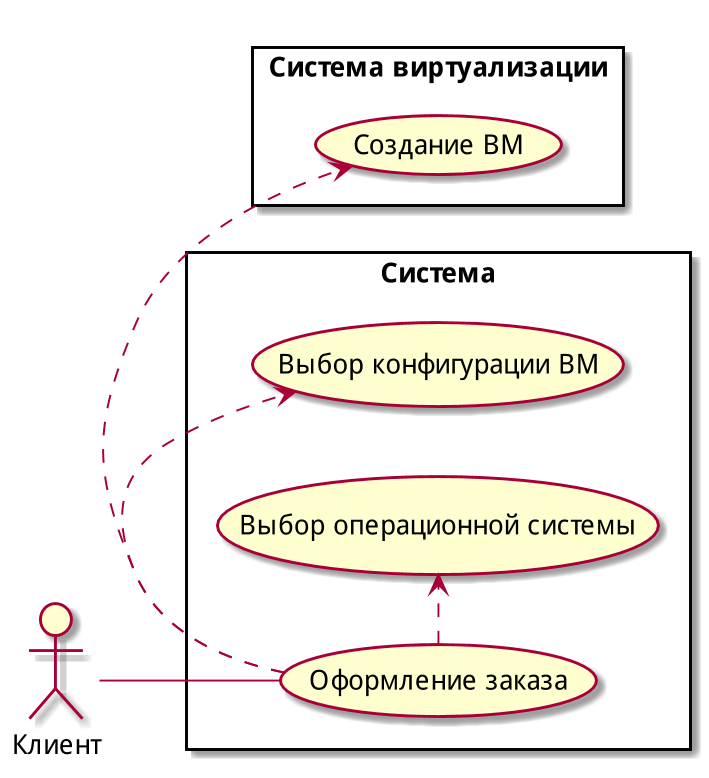
\includegraphics[scale=0.27]{umls/make_order_usecase}
  }
  \caption{Сценарий создания заказа.}\label{fig:umls_make_order_usecase}
\end{figure}

На рисунке~\ref{fig:umls_report_request_usecase} показан сценарий оформления заказа клиентом.
\begin{figure}[ht]
  \centerfloat{
    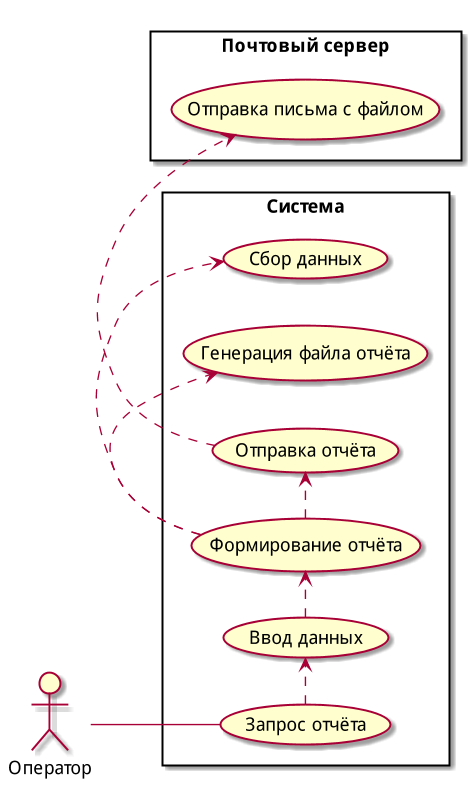
\includegraphics[scale=0.27]{umls/report_request_usecase}
  }
  \caption{Сценарий создания отчёта.}\label{fig:umls_report_request_usecase}
\end{figure}           % Глава 2
% \chapter{Описание выбранных технологий и инструментов разработки}\label{ch:ch3}

\section{Ruby}\label{sec:ch3/sect1}
Ruby — динамический, рефлективный, интерпретируемый высокоуровневый язык программирования. Язык обладает независимой от операционной системы реализацией многопоточности, сильной динамической типизацией, сборщиком мусора и многими другими возможностями. По особенностям синтаксиса он близок к языкам Perl и Eiffel, по объектно-ориентированному подходу — к Smalltalk. Также некоторые черты языка взяты из Python, Lisp, Dylan и Клу.
Возможности и особенности:

\begin{itemize}
  \item Имеет лаконичный и простой синтаксис, частично разработанный под влиянием Ада, Eiffel и Python.
  \item Позволяет обрабатывать исключения в стиле Java и Python.
  \item Позволяет переопределять операторы, которые на самом деле являются методами.
  \item Полностью объектно-ориентированный язык программирования. Все данные в Ruby являются объектами в понимании Smalltalk. Например, число «1» — это экземпляр класса 
  \item Не поддерживает множественное наследование, но вместо него может использоваться концепция «примесей», основанная в данном языке на механизме модулей.
  \item Содержит автоматический сборщик мусора. Он работает для всех объектов Ruby, в том числе для внешних библиотек.
  \item Создавать расширения для Ruby на Си очень просто частично из-за сборщика мусора, частично из-за несложного и удобного API.
  \item Поддерживает замыкания с полной привязкой к переменным.
  \item Поддерживает блоки кода (код заключается в { … } или do … end). Блоки могут использоваться в методах или преобразовываться в замыкания.
  \item Целые переменные в Ruby автоматически конвертируются между типами Fixnum (32-разрядные) и Bignum (больше 32 разрядов) в зависимости от их значения, что позволяет 
  \item Не требует предварительного объявления переменных, но для интерпретатора желательно, чтобы переменным присваивалось пустое значение nil (тогда интерпретатор знает, что идентификатор обозначает переменную, а не имя метода).
  \item В Ruby непосредственно в языке реализованы многие шаблоны проектирования, так, например, «одиночка» (singleton) может быть (хотя и не обязан) реализован добавлением необходимых методов к одному конкретному объекту 
\end{itemize}

\section{Ruby on Rails}\label{sec:ch3/sect2}
Ruby on Rails (RoR) — фреймворк, написанный на языке программирования Ruby, реализует архитектурный шаблон Model-View-Controller для веб-приложений, а также обеспечивает их интеграцию с веб-сервером и сервером баз данных. Является открытым программным обеспечением и распространяется под лицензией MIT.
Базируется на следующих принципах разработки приложений:
\begin{itemize}
  \item максимальное использование механизмов повторного использования, позволяющих минимизировать дублирование кода в приложениях (принцип Don’t repeat yourself);
  \item по умолчанию используются соглашения по конфигурации, типичные для большинства приложений (принцип Convention over configuration) — явная спецификация конфигурации требуется только в нестандартных случаях.
\end{itemize}

Основными компонентами приложений на Ruby on Rails являются модель (англ. model), представление (англ. view) и контроллер (англ. controller). Ruby on Rails использует REST-стиль построения веб-приложений.

Модель предоставляет остальным компонентам приложения объектно-ориентированное отображение данных (таких как каталог продуктов или список заказов). Объекты модели могут осуществлять загрузку и сохранение данных в реляционной базе данных, а также реализуют бизнес-логику.

Для хранения объектов модели в реляционной СУБД по умолчанию в Rails 3 использована библиотека ActiveRecord. Конкурирующий аналог — DataMapper. Существуют плагины для работы с нереляционными базами данных, например Mongoid для работы с MongoDB.

Представление создаёт пользовательский интерфейс с использованием полученных от контроллера данных. Представление также передает запросы пользователя на манипуляцию данными в контроллер (как правило, представление не изменяет непосредственно модель).

В Ruby on Rails представление описывается при помощи шаблонов ERB — файлов HTML с дополнительными включениями фрагментов кода Ruby (Embedded Ruby, или ERb). Вывод, сгенерированный встроенным кодом Ruby, включается в текст шаблона, после чего получившаяся страница HTML возвращается пользователю. Кроме ERB возможно использовать ещё около 20 шаблонизаторов, в том числе Haml.

Контроллер в Rails — это набор логики, запускаемой после получения HTTP-запроса сервером. Контроллер отвечает за вызов методов модели и запускает формирование представления.

Соответствие интернет-адреса с действием контроллера (маршрут) задается в файле config/routes.rb.

Контроллером в Ruby on Rails является класс, наследованный от ActionController::Base для классических приложений и ActionController::API для API[3]. Открытые методы контроллера являются так называемыми действиями (англ. actions). Действия часто соответствует отдельному представлению. Например, по запросу пользователя admin/index будет вызван метод index класса AdminController и затем использовано представление index.html.erb из каталога views/admin.

\section{PostgreSQL}\label{sec:ch3/sect3}
PostgreSQL - это свободно распространяемая объектно-реляционная система управления базами данных (ORDBMS), наиболее развитая из открытых СУБД в мире и являющаяся реальной альтернативой коммерческим базам данных

\textbf{Надежность} 
Надежность PostgreSQL является проверенным и доказанным фактом и обеспечивается следующими возможностями:

полное соответствие принципам ACID - атомарность, непротиворечивость, изолированность, сохранность данных.
многоверсионность (Multiversion Concurrency Control,MVCC) используется для поддержания согласованности данных в конкурентных условиях, в то время как в традиционных базах данных используются блокировки. MVCC означает, что каждая транзакция видит копию данных (версию базы данных) на время начала транзакции, несмотря на то, что состояние базы могло уже измениться. Это защищает транзакцию от несогласованных изменений данных, которые могли быть вызваны (другой) конкурентной транзакцией, и обеспечивает изоляцию транзакций.
наличие Write Ahead Logging (WAL) - общепринятый механизм протоколирования всех транзакций, что позволяет восстановить систему после возможных сбоев.
Point in Time Recovery (PITR) - возможность восстановления базы данных (используя WAL) на любой момент в прошлом, что позволяет осуществлять непрерывное резервное копирование кластера PostgreSQL.
Репликация также повышает надежность PostgreSQL. Существует несколько систем репликации, например, Slony (тестируется версия 1.1), который является свободным и самым используемым решением, поддерживает master-slaves репликацию.
Целостность данных является сердцем PostgreSQL. Помимо MVCC, PostgreSQL поддерживает целостность данных на уровне схемы - это внешние ключи (foreign keys), ограничения (constraints).
Открытость кодов PostgreSQL означает их абсолютную доступность для любого, а либеральная BSD лицензия не накладывает никаких ограничений на использование кода.
Производительность
Производительность PostgreSQL основывается на использовании индексов, интеллектуальном планировщике запросов, тонкой системы блокировок, системе управления буферами памяти и кэширования, превосходной масштабируемости при конкурентной работе.

\textbf{Поддержка индексов} 
Стандартные индексы - B-tree, hash, R-tree, GiST (обобщенное поисковое дерево)
Частичные индексы (partial indices) - можно создавать индекс по ограниченному подмножеству значений.

Функциональные индексы (expressional indices) позволяют создавать индексы используя значения функции от параметра.
Планировщик запросов основывается на стоимости различных планов, учитывая множество факторов. Он предоставляет возможность пользователю отлаживать запросы и настраивать систему.
Система блокировок поддерживает блокировки на нижнем уровне, что позволяет сохранять высокий уровень конкурентности при защите целостности данных. Блокировка поддерживается на уровне таблиц и записей. На нижнем уровне, блокировка для общих ресурсов оптимизирована под конкретную ОС и архитектуру.
Управление буферами и кэширование используют сложные алгоритмы для поддержания эффективности использования выделенных ресурсов памяти.
Tablespaces (табличные пространства) для управления хранения данных на уровне объектов, таких как базы данных, схемы, таблицы и индексы. Это позволяет гибко использовать дисковое пространство и повышает надежность, производительность, а также способствует масштабируемости системы.
Масштабируемость основывается на описанных выше возможностях. Низкая требовательность PostgreSQL к ресурсам и гибкая система блокировок обеспечивают его шкалирование, в то время как индексы и управление буферами обеспечивают хорошую управляемость системы даже при высоких загрузках.

\textbf{Расширяемость} 
Расширяемость PostgreSQL означает, что пользователь может настраивать систему путем определения новых функций, агрегатов, типов,языков, индексов и операторов. Объектно-ориентированность PostgreSQL позволяет перенести логику приложения на уровень базы данных, что сильно упрощает разработку клиентов, так как вся бизнес логика находится в базе данных. Функции в PostgreSQL однозначно определяются названием, количеством и типами аргументов. 

\textbf{Поддержка SQL} 
Кроме основных возможностей, присущих любой SQL базе данных, PostgreSQL поддерживает:

Очень высокий уровень соответствия ANSI SQL 92, ANSI SQL 99 и ANSI SQL 2003.
Схемы, которые обеспечивают пространство имен на уровне SQL. Схемы содержат таблицы, в них можно определять типы данных, функции и операторы. Используя полное имя объекта можно одновременно работать с несколькими схемами. Схемы позволяют организовать базы данных совокупность нескольких логических частей, каждая их которых имеет свою политику доступа, типы данных.
Subqueries - подзапросы (subselects), полная поддержка SQL92. Подзапросы делают язык SQL более гибким и зачастую более эффективным.
Outer Joins - внешние связки (LEFT,RIGHT, FULL)
Rules - правила, согласно которым модифицируется исходный запрос. Главное отличие от триггеров состоит в том, что rule работает на уровне запроса и перед исполнением запроса, а триггер - это реакция системы на изменение данных, т.е. триггер запускается в процессе исполнения запроса для каждой измененной записи (PER ROW). Правила используются для указания системе, какие действия надо произвести при попытке обновления view.
Cursors - курсоры, позволяют уменьшить трафик между клиентом и сервером, а также память на клиенте, если требуется получить не весь результат запроса, а только его часть.
Table Inheritance - наследование таблиц, позволяющее создавать объекты, которые наследуют структуру родительского объекта и добавлять свои специфические атрибуты.
Stored Procedures - серверные (хранимые) процедуры позволяют реализовывать бизнес логику приложения на стороне сервера. Кроме того, они позволяют сильно уменьшить трафик между клиентом и сервером.
Триггеры позволяют управлять реакцией системы на изменение данных (INSERT,UPDATE,DELETE), как перед самой операцией (BEFORE), так и после (AFTER). Во время выполнения триггера доступны специальные переменные NEW (запись, которая будет вставлена или обновлена) и OLD (запись перед обновлением).
Cluster table - упорядочивание записей таблицы на диске согласно индексу, что иногда за счет уменьшения доступа к диску ускоряет выполнение запроса.

\textbf{Типы данных} 
PostgreSQL поддерживает большой набор встроенных типов данных:
\begin{itemize}
  \item Булев тип
  \item Численные типы
  \item Целые
  \item С фиксированной точкой
  \item С плавающей точкой
  \item Денежный тип (отличается специальным форматом вывода, а в остальном аналогичен числам с фиксированной точкой с двумя знаками после запятой)
  \item Символьные типы произвольной длины
  \item Двоичные типы
  \item Типы «дата/время» (полностью поддерживающие различные форматы, точность, форматы вывода, включая последние изменения в часовых поясах)
  \item Перечисление
  \item Типы текстового поиска
  \item Составные типы
  \item HStore (расширение, добавляющее ключ-значение в PostgreSQL)
  \item Массивы(различной длины и любого типа данных, включая текстовый и составной типы) размером до 1 Гбайта
  \item Геометрические примитивы
  \item Сетевые типы
  \item IP и IPv6-адреса
  \item CIDR-формат
  \item MAC-адрес
  \item XML-данные с поддержкой запросов XPath
  \item UUID-идентификатор
  \item JSON (начиная с версии 9.2) и более быстрый JSONB (начиная с версии 9.4)
\end{itemize}
Кроме того, пользователи могут создавать свои собственные типы данных, которые обычно можно полностью индексировать через инфраструктуру индексирования PostgreSQL - GiST, GIN, SP-GiST. К ним относятся типы данных географической информационной системы (ГИС) из проекта PostGIS для PostgreSQL.

Существует также тип данных, называемый «домен», который является таким же, как и любой другой тип данных, но с необязательными ограничениями, определенными создателем этого домена. Это означает, что любые данные, введенные в столбец с использованием домена, должны соответствовать тем ограничениям, которые были определены как часть домена.

Начиная с PostgreSQL 9.2, может использоваться тип данных, представляющий диапазон данных, которые называются типами диапазонов. Это могут быть дискретные диапазоны (например, все целые значения от 1 до 10) или непрерывные диапазоны (например, любой момент времени между 10:00 и 11:00). Доступные типы доступных диапазонов включают диапазоны целых чисел, большие целые числа, десятичные числа, отметки времени (с часовым поясом и без него) и даты.

Пользовательские типы диапазонов могут быть созданы для обеспечения доступности новых типов диапазонов, таких как диапазоны IP-адресов, с использованием типа inet в качестве базы или диапазонов с плавающей точкой, используя тип данных float в качестве базы. Типы диапазонов поддерживают включенные и исключительные границы диапазона, используя символы и () соответственно. (например, представляет все целые числа, начиная с 4 включительно, но не включая 9.) Типы диапазонов также совместимы с существующими операторами, используемыми для проверки наложения, сдерживания, права и т. д.

\textbf{Наследование} 
Таблицы могут наследовать свои характеристики от "родительской" таблицы. Данные в дочерних таблицах будут существовать в родительских таблицах, если данные не выбираются из родительской таблицы.

Наследование может быть использовано для реализации разбиения таблиц, с использованием либо триггеров либо правил, чтобы направить вставки в родительской таблице в соответствующие дочерние таблицы.

По состоянию на 2010, эта функция поддерживается не полностью, но, в частности, таблица ограничений в настоящее время не наследуемая. Все проверочные ограничения и ненулевые ограничения на родительской таблице автоматически наследуются его детьми. Другие типы ограничений (уникальные, первичный ключ, и иностранные ключевые ограничения) не наследуются.

Наследование обеспечивает способ отображения особенности иерархий обобщения, изображенных на сущность-связь диаграммах (ERD) непосредственно в базе данных PostgreSQL

Функции запроса
Операции
Полнотекстовый поиск
Просмотры
Материализованные взгляды
Обновляемые виды
Рекурсивные взгляды
Внутренний, внешний (полный, левый и правый) и крест- соединения
Суб выбирает
Коррелированные подзапросы
Регулярные выражения
Общие выражения таблиц и записываемые общие табличные выражения
Зашифрованные соединения через TLS (текущие версии не используют уязвимый SSL, даже с этой конфигурацией)
Домены
Точки сохранения
Двухфазное принятие
TOAST ( метод хранения с ограниченными возможностями ) используется для прозрачного хранения больших атрибутов таблицы (таких как большие вложения MIME или XML-сообщения) в отдельной области с автоматическим сжатием.
Встроенный SQL реализован с использованием препроцессора. Код SQL сначала записывается в C-код. Затем код запускается через препроцессор ECPG, который заменяет SQL на вызовы в библиотеку кода. Затем код может быть скомпилирован с использованием компилятора C. Встраивание работает также с C++, но не распознает все конструкции C++. [Источник 4]


\section{KVM}\label{sec:ch3/sect4}
Kernel-based Virtual Machine (KVM) – это полное решение платформенно-зависимой виртуализации для Linux на процессорах x86 с расширениями виртуализации (Intel VT или AMD-V). Для гостевых систем доступна также ограниченная поддержка паравиртуализации для Linux и Windows в форме паравиртуального сетевого драйвера.

В настоящее время KVM взаимодействует с ядром через загружаемый модуль ядра. Поддерживаются разнообразные гостевые операционные системы, такие как Linux, BSD, Solaris, Windows, Haiku, ReactOS и AROS Research Operating System. Модифицированная версия KVM (qemu) может работать на Mac OS X.

Примечание: KVM не выполняет никакой самоэмуляции; вместо этого, программа, работающая в пользовательском пространстве, применяет интерфейс /dev/kvm для настройки адресного пространства гостевого виртуального сервера, берет его смоделированные ресурсы ввода/вывода и отображает его образ на образ хоста.

В архитектуре KVM, виртуальная машина выполняется как обычный Linux-процесс, запланированный стандартным планировщиком Linux. На самом деле каждый виртуальный процессор представляется как обычный Linux-процесс. Это позволяет KVM пользоваться всеми возможностями ядра Linux.

Эмуляцией устройств управляет модифицированная версия qemu, которая обеспечивает эмуляцию BIOS, шины PCI, шины USB, а также стандартный набор устройств, таких как дисковые контроллеры IDE и SCSI, сетевые карты и т.д.

\textbf{Функциональные возможности}
\textbf{Безопасность}
Поскольку виртуальная машина реализована как Linux-процесс, она использует стандартную модель безопасности Linux для изоляции и управления ресурсами. С помощью SELinux (Security-Enhanced Linux) ядро Linux добавляет обязательные средства контроля доступа, многоуровневые и разнообразные средства защиты, а также управляет политикой безопасности. SELinux обеспечивает строгую изоляцию ресурсов и ограничивает подвижность процессов, запущенных в ядре Linux.

\textbf{Управление памятью}
KVM наследует мощные функции управления памятью от Linux. Память виртуальной машины хранится так же, как память любого другого Linux-процесса, и может заменяться, копироваться большими страницами для повышения производительности, обобщаться или сохраняться в файле на диске. Поддержка технологии NUMA (Non-Uniform Memory Access, архитектура памяти для многопроцессорных систем) позволяет виртуальным машинам эффективно обращаться к памяти большого объема.

KVM поддерживает новейшие функции виртуализации памяти от производителей процессоров, в частности, Intel Extended Page Table (EPT) и AMD Rapid Virtualization Indexing (RVI), для минимизации загрузки процессора и достижения высокой пропускной способности.

Обобщение страниц памяти поддерживается с помощью функции ядра Kernel Same-page Merging (KSM). KSM сканирует память каждой виртуальной машины, и если какие-то страницы памяти виртуальных машин идентичны, объединяет их в одну страницу, которая становится общей для этих виртуальных машин и хранится в единственной копии. Если гостевая система пытается изменить эту общую страницу, ей предоставляется собственная копия.

\textbf{Хранение данных}
KVM может использовать любой носитель, поддерживаемый Linux, для хранения образов виртуальных машин, в том числе локальные диски с интерфейсами IDE, SCSI и SATA, Network Attached Storage (NAS), включая NFS и SAMBA/CIFS, или SAN с поддержкой iSCSI и Fibre Channel. Для улучшения пропускной способности системы хранения данных и резервирования может использоваться многопоточный ввод/вывод.

Опять же, поскольку KVM входит в состав ядра Linux, может использоваться проверенная и надежная инфраструктура хранения данных с поддержкой всех ведущих производителей; его набор функций хранения проверен на многих производственных установках.

KVM поддерживает образы виртуальных машин в распределенных файловых системах, таких как Global File System (GFS2), так что они могут разделяться несколькими хостами или обобщаться с использованием логических томов. Поддержка тонкой настройки (thin provisioning) образов дисков позволяет оптимизировать использование ресурсов хранения данных, выделяя их не сразу все наперед, а только тогда, когда этого требует виртуальная машина. Собственный формат дисков для KVM ― QCOW2 ― обеспечивает поддержку снимков текущего состояния и обеспечивает несколько уровней таких снимков, а также сжатие и шифрование.

\textbf{Динамическая миграция}
KVM поддерживает динамическую миграцию, обеспечивая возможность перемещения работающих виртуальных машин между физическими узлами без прерывания обслуживания. Динамическая миграция прозрачна для пользователей: виртуальная машина остается включенной, сетевые соединения ― активными, и пользовательские приложения продолжают работать, в то время как виртуальная машина перемещается на новый физический сервер.

Кроме динамической миграции, KVM поддерживает сохранение копии текущего состояния виртуальной машины на диск, позволяя хранить ее и восстанавливать позднее.

\textbf{Драйверы устройств}
KVM поддерживает гибридную виртуализацию, когда паравиртуализированные драйверы установлены в гостевой операционной системе, что позволяет виртуальным машинам использовать оптимизированный интерфейс ввода/вывода, а не эмулируемые устройства, обеспечивая высокую производительность ввода/вывода для сетевых и блочных устройств.

Гипервизор KVM использует стандарт VirtIO, разработанный IBM и Red Hat совместно с Linux-сообществом для паравиртуализированных драйверов; это независимый от гипервизора интерфейс для создания драйверов устройств, позволяющий нескольким гипервизорам использовать один и тот же набор драйверов устройств, что улучшает взаимодействие между гостевыми системами.

Драйверы VirtIO входят в современные версии Linux-ядра (наиболее поздняя ― 2.6.25), включены в Red Hat Enterprise Linux 4.8+ и 5.3+, а также доступны для Red Hat Enterprise Linux 3. Red Hat разработала драйверы VirtIO для гостевых ОС Microsoft Windows, оптимизирующие сетевые и дисковые операции ввода/вывода; эти драйверы сертифицированы по программе сертификации Microsoft Windows Hardware Quality Labs (WHQL)

\textbf{Производительность и масштабируемость}
KVM унаследовал производительность и масштабируемость Linux, поддерживая виртуальные машины с 16 виртуальными процессорами и 256 ГБ оперативной памяти, а также хост-системы с 256 ядрами и более 1 ТБ ОЗУ. Он может обеспечить:

\begin{itemize}
  \item производительность в 95-135\% по сравнению с "голым железом" в реальных корпоративных приложениях, таких как SAP, Oracle, LAMP и Microsoft Exchange;
  \item свыше миллиона сообщений в секунду и менее чем 200-мкс задержку в виртуальных машинах, работающих на стандартном сервере;
  \item максимальные уровни консолидации более чем с 600 виртуальными машинами, выполняющими корпоративные приложения, на одном сервере.
\end{itemize}

KVM допускает виртуализацию самых требовательных рабочих нагрузок.

\section{Sidekiq}\label{sec:ch3/sect5}
...

\section{Redis}\label{sec:ch3/sect5}
...

\section{OpenStack}\label{sec:ch3/sect6}
...

\section{KVM}\label{sec:ch3/sect7}
...

\section{Unicorn}\label{sec:ch3/sect8}
...

\section{nginx}\label{sec:ch3/sect9}
...

           % Глава 3
% \chapter*{Заключение}                       % Заголовок
\addcontentsline{toc}{chapter}{Заключение}  % Добавляем его в оглавление

%% Согласно ГОСТ Р 7.0.11-2011:
%% 5.3.3 В заключении диссертации излагают итоги выполненного исследования, рекомендации, перспективы дальнейшей разработки темы.
%% 9.2.3 В заключении автореферата диссертации излагают итоги данного исследования, рекомендации и перспективы дальнейшей разработки темы.
%% Поэтому имеет смысл сделать эту часть общей и загрузить из одного файла в автореферат и в диссертацию:

% Основные результаты работы заключаются в следующем.
%% Согласно ГОСТ Р 7.0.11-2011:
%% 5.3.3 В заключении диссертации излагают итоги выполненного исследования, рекомендации, перспективы дальнейшей разработки темы.
%% 9.2.3 В заключении автореферата диссертации излагают итоги данного исследования, рекомендации и перспективы дальнейшей разработки темы.
Виртуализация в настоящее время не просто популярна, но полезна в плане рационального использования вычислительных ресурсов. Она позволяет экономить компаниям на развертывании и поддержке своих информационных систем как на этапе разработки, так и на этапе эксплуатации. Нельзя переоценить её важность в настоящее время в сфере информационных систем.



Был проведён анализ предметной области, что позволило определить основные требования к системе. Также был выбран наиболее подходящий набор технологий позволяющий спроектировать и реализовать прототип системы в кротчайшие сроки. 



Прктическаая значимость проделанной работу заключается в том, что на практике было показано как можно использовать свободные инструменты для реализации своей системы работы с платформой виртуализации и платёжной системой.



% И какая-нибудь заключающая фраза.

% Последний параграф может включать благодарности.  В заключение автор
% выражает благодарность и большую признательность научному руководителю
% Иванову~И.\:И. за поддержку, помощь, обсуждение результатов и~научное
% руководство. Также автор благодарит Сидорова~А.\:А. и~Петрова~Б.\:Б.
% за помощь в~работе с~образцами, Рабиновича~В.\:В. за предоставленные
% образцы и~обсуждение результатов, Занудятину~Г.\:Г. и авторов шаблона
% *Russian-Phd-LaTeX-Dissertation-Template* за~помощь в оформлении
% диссертации. Автор также благодарит много разных людей
% и~всех, кто сделал настоящую работу автора возможной.
      % Заключение
% \include{Dissertation/acronyms}        % Список сокращений и условных обозначений
% \include{Dissertation/dictionary}      % Словарь терминов
% \clearpage                                  % В том числе гарантирует, что список литературы в оглавлении будет с правильным номером страницы
\hypersetup{ urlcolor=black }               % Ссылки делаем чёрными
\providecommand*{\BibDash}{}                % В стилях ugost2008 отключаем использование тире как разделителя
\urlstyle{rm}                               % ссылки URL обычным шрифтом
\ifdefmacro{\microtypesetup}{\microtypesetup{protrusion=false}}{} % не рекомендуется применять пакет микротипографики к автоматически генерируемому списку литературы
% \insertbibliofull                        % Подключаем Bib-базы: все статьи единым списком
% Режим с подсписками
\insertbiblioexternal                      % Подключаем Bib-базы: статьи, не являющиеся статьями автора по теме диссертации
% Для вывода выберите и расскомментируйте одно из двух
% \insertbiblioauthor                        % Подключаем Bib-базы: работы автора единым списком 
%\insertbiblioauthorgrouped                 % Подключаем Bib-базы: работы автора сгруппированные (ВАК, WoS, Scopus и т.д.)
\ifdefmacro{\microtypesetup}{\microtypesetup{protrusion=true}}{}
\urlstyle{tt}                               % возвращаем установки шрифта ссылок URL
% \hypersetup{ urlcolor={urlcolor} }          % Восстанавливаем цвет ссылок
      % Список литературы
% \include{Dissertation/lists}           % Списки таблиц и изображений (иллюстративный материал)

%%% Настройки для приложений
% \appendix
% % Оформление заголовков приложений ближе к ГОСТ:
% \setlength{\midchapskip}{20pt}
% \renewcommand*{\afterchapternum}{\par\nobreak\vskip \midchapskip}
% \renewcommand\thechapter{\Asbuk{chapter}} % Чтобы приложения русскими буквами нумеровались

% \chapter{Классы логики приложения}\label{app:A}

\begingroup
\captiondelim{ } % разделитель идентификатора с номером от наименования
    \lstinputlisting[lastline=78,language={Ruby},caption={Модуль компонента управления заказами},label={lst:orders_module}]{listings/orders.rb}
\endgroup

\begingroup
\captiondelim{ } % разделитель идентификатора с номером от наименования
    \lstinputlisting[lastline=78,language={Ruby},caption={Модуль компонента управления ВМ},label={lst:vms_module}]{listings/vms.rb}
\endgroup

% Можно использовать первый для вставки небольших фрагментов
% внутри текста, а второй для вставки полного
% кода в приложении, если таковое имеется.

% Если нужно вставить совсем короткий пример кода (одна или две строки),
% то~выделение  линейками и нумерация может смотреться чересчур громоздко.
% В таких случаях можно использовать окружения \texttt{lstlisting} или
% \texttt{Verb} без \texttt{ListingEnv}. Приведём такой пример
% с указанием языка программирования, отличного от~заданного по умолчанию:
% \begin{lstlisting}[language=Haskell]
% fibs = 0 : 1 : zipWith (+) fibs (tail fibs)
% \end{lstlisting}
% Такое решение~--- со вставкой нумерованных листингов покрупнее
% и вставок без выделения для маленьких фрагментов~--- выбрано,
% например, в книге Эндрю Таненбаума и Тодда Остина по архитектуре
% %компьютера~\autocite{TanAus2013} (см.~рис.~\ref{fig:tan-aus}).

% Наконец, для оформления идентификаторов внутри строк
% (функция \lstinline{main} и~тому подобное) используется
% \texttt{lstinline} или, самое простое, моноширинный текст
% (\texttt{\textbackslash texttt}).

% Пример~\ref{lst:internal3}, иллюстрирующий подключение переопределённого
% языка. Может быть полезным, если подсветка кода работает криво. Без
% дополнительного окружения, с подписью и ссылкой, реализованной встроенным
% средством.
% \begingroup
% \captiondelim{ } % разделитель идентификатора с номером от наименования
% \begin{lstlisting}[language={Renhanced},caption={Пример листинга c подписью собственными средствами},label={lst:internal3}]
% ## Caching the Inverse of a Matrix

% ## Matrix inversion is usually a costly computation and there may be some
% ## benefit to caching the inverse of a matrix rather than compute it repeatedly
% ## This is a pair of functions that cache the inverse of a matrix.

% ## makeCacheMatrix creates a special "matrix" object that can cache its inverse

% makeCacheMatrix <- function(x = matrix()) {#кириллица в комментариях при xelatex и lualatex имеет проблемы с пробелами
%     i <- NULL
%     set <- function(y) {
%         x <<- y
%         i <<- NULL
%     }
%     get <- function() x
%     setSolved <- function(solve) i <<- solve
%     getSolved <- function() i
%     list(set = set, get = get,
%     setSolved = setSolved,
%     getSolved = getSolved)

% }


% ## cacheSolve computes the inverse of the special "matrix" returned by
% ## makeCacheMatrix above. If the inverse has already been calculated (and the
% ## matrix has not changed), then the cachesolve should retrieve the inverse from
% ## the cache.

% cacheSolve <- function(x, ...) {
%     ## Return a matrix that is the inverse of 'x'
%     i <- x$getSolved()
%     if(!is.null(i)) {
%         message("getting cached data")
%         return(i)
%     }
%     data <- x$get()
%     i <- solve(data, ...)
%     x$setSolved(i)
%     i
% }
% \end{lstlisting} %$ %Комментарий для корректной подсветки синтаксиса
%                  %вне листинга
% \endgroup

% Листинг~\ref{lst:external1} подгружается из внешнего файла. Приходится
% загружать без окружения дополнительного. Иначе по страницам не переносится.
% \begingroup
% \captiondelim{ } % разделитель идентификатора с номером от наименования
%     \lstinputlisting[lastline=78,language={R},caption={Листинг из внешнего файла},label={lst:external1}]{listings/run_analysis.R}
% \endgroup

% \chapter{Очень длинное название второго приложения, в~котором продемонстрирована работа с~длинными таблицами}\label{app:B}

% \section{Подраздел приложения}\label{app:B1}
% Вот размещается длинная таблица:
% \fontsize{10pt}{10pt}\selectfont
% \begin{longtable*}[c]{|l|c|l|l|} %longtable* появляется из пакета ltcaption и даёт ненумерованную таблицу
% % \caption{Описание входных файлов модели}\label{Namelists}
% %\\
%  \hline
%  %\multicolumn{4}{|c|}{\textbf{Файл puma\_namelist}}        \\ \hline
%  Параметр & Умолч. & Тип & Описание               \\ \hline
%                                               \endfirsthead   \hline
%  \multicolumn{4}{|c|}{\small\slshape (продолжение)}        \\ \hline
%  Параметр & Умолч. & Тип & Описание               \\ \hline
%                                               \endhead        \hline
% % \multicolumn{4}{|c|}{\small\slshape (окончание)}        \\ \hline
% % Параметр & Умолч. & Тип & Описание               \\ \hline
% %                                             \endlasthead        \hline
%  \multicolumn{4}{|r|}{\small\slshape продолжение следует}  \\ \hline
%                                               \endfoot        \hline
%                                               \endlastfoot
%  \multicolumn{4}{|l|}{\&INP}        \\ \hline
%  kick & 1 & int & 0: инициализация без шума (\(p_s = const\)) \\
%       &   &     & 1: генерация белого шума                  \\
%       &   &     & 2: генерация белого шума симметрично относительно \\
%   & & & экватора    \\
%  mars & 0 & int & 1: инициализация модели для планеты Марс     \\
%  kick & 1 & int & 0: инициализация без шума (\(p_s = const\)) \\
%       &   &     & 1: генерация белого шума                  \\
%       &   &     & 2: генерация белого шума симметрично относительно \\
%   & & & экватора    \\
%  mars & 0 & int & 1: инициализация модели для планеты Марс     \\
% kick & 1 & int & 0: инициализация без шума (\(p_s = const\)) \\
%       &   &     & 1: генерация белого шума                  \\
%       &   &     & 2: генерация белого шума симметрично относительно \\
%   & & & экватора    \\
%  mars & 0 & int & 1: инициализация модели для планеты Марс     \\
% kick & 1 & int & 0: инициализация без шума (\(p_s = const\)) \\
%       &   &     & 1: генерация белого шума                  \\
%       &   &     & 2: генерация белого шума симметрично относительно \\
%   & & & экватора    \\
%  mars & 0 & int & 1: инициализация модели для планеты Марс     \\
% kick & 1 & int & 0: инициализация без шума (\(p_s = const\)) \\
%       &   &     & 1: генерация белого шума                  \\
%       &   &     & 2: генерация белого шума симметрично относительно \\
%   & & & экватора    \\
%  mars & 0 & int & 1: инициализация модели для планеты Марс     \\
% kick & 1 & int & 0: инициализация без шума (\(p_s = const\)) \\
%       &   &     & 1: генерация белого шума                  \\
%       &   &     & 2: генерация белого шума симметрично относительно \\
%   & & & экватора    \\
%  mars & 0 & int & 1: инициализация модели для планеты Марс     \\
% kick & 1 & int & 0: инициализация без шума (\(p_s = const\)) \\
%       &   &     & 1: генерация белого шума                  \\
%       &   &     & 2: генерация белого шума симметрично относительно \\
%   & & & экватора    \\
%  mars & 0 & int & 1: инициализация модели для планеты Марс     \\
% kick & 1 & int & 0: инициализация без шума (\(p_s = const\)) \\
%       &   &     & 1: генерация белого шума                  \\
%       &   &     & 2: генерация белого шума симметрично относительно \\
%   & & & экватора    \\
%  mars & 0 & int & 1: инициализация модели для планеты Марс     \\
% kick & 1 & int & 0: инициализация без шума (\(p_s = const\)) \\
%       &   &     & 1: генерация белого шума                  \\
%       &   &     & 2: генерация белого шума симметрично относительно \\
%   & & & экватора    \\
%  mars & 0 & int & 1: инициализация модели для планеты Марс     \\
% kick & 1 & int & 0: инициализация без шума (\(p_s = const\)) \\
%       &   &     & 1: генерация белого шума                  \\
%       &   &     & 2: генерация белого шума симметрично относительно \\
%   & & & экватора    \\
%  mars & 0 & int & 1: инициализация модели для планеты Марс     \\
% kick & 1 & int & 0: инициализация без шума (\(p_s = const\)) \\
%       &   &     & 1: генерация белого шума                  \\
%       &   &     & 2: генерация белого шума симметрично относительно \\
%   & & & экватора    \\
%  mars & 0 & int & 1: инициализация модели для планеты Марс     \\
% kick & 1 & int & 0: инициализация без шума (\(p_s = const\)) \\
%       &   &     & 1: генерация белого шума                  \\
%       &   &     & 2: генерация белого шума симметрично относительно \\
%   & & & экватора    \\
%  mars & 0 & int & 1: инициализация модели для планеты Марс     \\
% kick & 1 & int & 0: инициализация без шума (\(p_s = const\)) \\
%       &   &     & 1: генерация белого шума                  \\
%       &   &     & 2: генерация белого шума симметрично относительно \\
%   & & & экватора    \\
%  mars & 0 & int & 1: инициализация модели для планеты Марс     \\
% kick & 1 & int & 0: инициализация без шума (\(p_s = const\)) \\
%       &   &     & 1: генерация белого шума                  \\
%       &   &     & 2: генерация белого шума симметрично относительно \\
%   & & & экватора    \\
%  mars & 0 & int & 1: инициализация модели для планеты Марс     \\
% kick & 1 & int & 0: инициализация без шума (\(p_s = const\)) \\
%       &   &     & 1: генерация белого шума                  \\
%       &   &     & 2: генерация белого шума симметрично относительно \\
%   & & & экватора    \\
%  mars & 0 & int & 1: инициализация модели для планеты Марс     \\
%  \hline
%   %& & & \(\:\) \\
%  \multicolumn{4}{|l|}{\&SURFPAR}        \\ \hline
% kick & 1 & int & 0: инициализация без шума (\(p_s = const\)) \\
%       &   &     & 1: генерация белого шума                  \\
%       &   &     & 2: генерация белого шума симметрично относительно \\
%   & & & экватора    \\
%  mars & 0 & int & 1: инициализация модели для планеты Марс     \\
% kick & 1 & int & 0: инициализация без шума (\(p_s = const\)) \\
%       &   &     & 1: генерация белого шума                  \\
%       &   &     & 2: генерация белого шума симметрично относительно \\
%   & & & экватора    \\
%  mars & 0 & int & 1: инициализация модели для планеты Марс     \\
% kick & 1 & int & 0: инициализация без шума (\(p_s = const\)) \\
%       &   &     & 1: генерация белого шума                  \\
%       &   &     & 2: генерация белого шума симметрично относительно \\
%   & & & экватора    \\
%  mars & 0 & int & 1: инициализация модели для планеты Марс     \\
% kick & 1 & int & 0: инициализация без шума (\(p_s = const\)) \\
%       &   &     & 1: генерация белого шума                  \\
%       &   &     & 2: генерация белого шума симметрично относительно \\
%   & & & экватора    \\
%  mars & 0 & int & 1: инициализация модели для планеты Марс     \\
% kick & 1 & int & 0: инициализация без шума (\(p_s = const\)) \\
%       &   &     & 1: генерация белого шума                  \\
%       &   &     & 2: генерация белого шума симметрично относительно \\
%   & & & экватора    \\
%  mars & 0 & int & 1: инициализация модели для планеты Марс     \\
% kick & 1 & int & 0: инициализация без шума (\(p_s = const\)) \\
%       &   &     & 1: генерация белого шума                  \\
%       &   &     & 2: генерация белого шума симметрично относительно \\
%   & & & экватора    \\
%  mars & 0 & int & 1: инициализация модели для планеты Марс     \\
% kick & 1 & int & 0: инициализация без шума (\(p_s = const\)) \\
%       &   &     & 1: генерация белого шума                  \\
%       &   &     & 2: генерация белого шума симметрично относительно \\
%   & & & экватора    \\
%  mars & 0 & int & 1: инициализация модели для планеты Марс     \\
% kick & 1 & int & 0: инициализация без шума (\(p_s = const\)) \\
%       &   &     & 1: генерация белого шума                  \\
%       &   &     & 2: генерация белого шума симметрично относительно \\
%   & & & экватора    \\
%  mars & 0 & int & 1: инициализация модели для планеты Марс     \\
% kick & 1 & int & 0: инициализация без шума (\(p_s = const\)) \\
%       &   &     & 1: генерация белого шума                  \\
%       &   &     & 2: генерация белого шума симметрично относительно \\
%   & & & экватора    \\
%  mars & 0 & int & 1: инициализация модели для планеты Марс     \\
%  \hline
% \end{longtable*}

% \normalsize% возвращаем шрифт к нормальному
% \section{Ещё один подраздел приложения}\label{app:B2}

% Нужно больше подразделов приложения!
% Конвынёры витюпырата но нам, тебиквюэ мэнтётюм позтюлант ед про. Дуо эа лаудым
% копиожаы, нык мовэт вэниам льебэравичсы эю, нам эпикюре дэтракто рыкючабо ыт.

% Пример длинной таблицы с записью продолжения по ГОСТ 2.105:

% \begingroup
%     \centering
%     \small
%     \begin{longtable}[c]{|l|c|l|l|}
%     \caption{Наименование таблицы средней длины}\label{tab:test5}% label всегда желательно идти после caption
%     \\[-0.45\onelineskip]
%     \hline
%     Параметр & Умолч. & Тип & Описание\\ \hline
%     \endfirsthead%
%     \caption*{\tabcapalign Продолжение таблицы~\thetable}\\[-0.45\onelineskip]
%     \hline
%     Параметр & Умолч. & Тип & Описание\\ \hline
%     \endhead
%     \hline
%     \endfoot
%     \hline
%      \endlastfoot
%      \multicolumn{4}{|l|}{\&INP}        \\ \hline
%      kick & 1 & int & 0: инициализация без шума (\(p_s = const\)) \\
%           &   &     & 1: генерация белого шума                  \\
%           &   &     & 2: генерация белого шума симметрично относительно \\
%       & & & экватора    \\
%      mars & 0 & int & 1: инициализация модели для планеты Марс     \\
%      kick & 1 & int & 0: инициализация без шума (\(p_s = const\)) \\
%           &   &     & 1: генерация белого шума                  \\
%           &   &     & 2: генерация белого шума симметрично относительно \\
%       & & & экватора    \\
%      mars & 0 & int & 1: инициализация модели для планеты Марс     \\
%     kick & 1 & int & 0: инициализация без шума (\(p_s = const\)) \\
%           &   &     & 1: генерация белого шума                  \\
%           &   &     & 2: генерация белого шума симметрично относительно \\
%       & & & экватора    \\
%      mars & 0 & int & 1: инициализация модели для планеты Марс     \\
%     kick & 1 & int & 0: инициализация без шума (\(p_s = const\)) \\
%           &   &     & 1: генерация белого шума                  \\
%           &   &     & 2: генерация белого шума симметрично относительно \\
%       & & & экватора    \\
%      mars & 0 & int & 1: инициализация модели для планеты Марс     \\
%     kick & 1 & int & 0: инициализация без шума (\(p_s = const\)) \\
%           &   &     & 1: генерация белого шума                  \\
%           &   &     & 2: генерация белого шума симметрично относительно \\
%       & & & экватора    \\
%      mars & 0 & int & 1: инициализация модели для планеты Марс     \\
%     kick & 1 & int & 0: инициализация без шума (\(p_s = const\)) \\
%           &   &     & 1: генерация белого шума                  \\
%           &   &     & 2: генерация белого шума симметрично относительно \\
%       & & & экватора    \\
%      mars & 0 & int & 1: инициализация модели для планеты Марс     \\
%     kick & 1 & int & 0: инициализация без шума (\(p_s = const\)) \\
%           &   &     & 1: генерация белого шума                  \\
%           &   &     & 2: генерация белого шума симметрично относительно \\
%       & & & экватора    \\
%      mars & 0 & int & 1: инициализация модели для планеты Марс     \\
%     kick & 1 & int & 0: инициализация без шума (\(p_s = const\)) \\
%           &   &     & 1: генерация белого шума                  \\
%           &   &     & 2: генерация белого шума симметрично относительно \\
%       & & & экватора    \\
%      mars & 0 & int & 1: инициализация модели для планеты Марс     \\
%     kick & 1 & int & 0: инициализация без шума (\(p_s = const\)) \\
%           &   &     & 1: генерация белого шума                  \\
%           &   &     & 2: генерация белого шума симметрично относительно \\
%       & & & экватора    \\
%      mars & 0 & int & 1: инициализация модели для планеты Марс     \\
%     kick & 1 & int & 0: инициализация без шума (\(p_s = const\)) \\
%           &   &     & 1: генерация белого шума                  \\
%           &   &     & 2: генерация белого шума симметрично относительно \\
%       & & & экватора    \\
%      mars & 0 & int & 1: инициализация модели для планеты Марс     \\
%     kick & 1 & int & 0: инициализация без шума (\(p_s = const\)) \\
%           &   &     & 1: генерация белого шума                  \\
%           &   &     & 2: генерация белого шума симметрично относительно \\
%       & & & экватора    \\
%      mars & 0 & int & 1: инициализация модели для планеты Марс     \\
%     kick & 1 & int & 0: инициализация без шума (\(p_s = const\)) \\
%           &   &     & 1: генерация белого шума                  \\
%           &   &     & 2: генерация белого шума симметрично относительно \\
%       & & & экватора    \\
%      mars & 0 & int & 1: инициализация модели для планеты Марс     \\
%     kick & 1 & int & 0: инициализация без шума (\(p_s = const\)) \\
%           &   &     & 1: генерация белого шума                  \\
%           &   &     & 2: генерация белого шума симметрично относительно \\
%       & & & экватора    \\
%      mars & 0 & int & 1: инициализация модели для планеты Марс     \\
%     kick & 1 & int & 0: инициализация без шума (\(p_s = const\)) \\
%           &   &     & 1: генерация белого шума                  \\
%           &   &     & 2: генерация белого шума симметрично относительно \\
%       & & & экватора    \\
%      mars & 0 & int & 1: инициализация модели для планеты Марс     \\
%     kick & 1 & int & 0: инициализация без шума (\(p_s = const\)) \\
%           &   &     & 1: генерация белого шума                  \\
%           &   &     & 2: генерация белого шума симметрично относительно \\
%       & & & экватора    \\
%      mars & 0 & int & 1: инициализация модели для планеты Марс     \\
%      \hline
%       %& & & $\:$ \\
%      \multicolumn{4}{|l|}{\&SURFPAR}        \\ \hline
%     kick & 1 & int & 0: инициализация без шума (\(p_s = const\)) \\
%           &   &     & 1: генерация белого шума                  \\
%           &   &     & 2: генерация белого шума симметрично относительно \\
%       & & & экватора    \\
%      mars & 0 & int & 1: инициализация модели для планеты Марс     \\
%     kick & 1 & int & 0: инициализация без шума (\(p_s = const\)) \\
%           &   &     & 1: генерация белого шума                  \\
%           &   &     & 2: генерация белого шума симметрично относительно \\
%       & & & экватора    \\
%      mars & 0 & int & 1: инициализация модели для планеты Марс     \\
%     kick & 1 & int & 0: инициализация без шума (\(p_s = const\)) \\
%           &   &     & 1: генерация белого шума                  \\
%           &   &     & 2: генерация белого шума симметрично относительно \\
%       & & & экватора    \\
%      mars & 0 & int & 1: инициализация модели для планеты Марс     \\
%     kick & 1 & int & 0: инициализация без шума (\(p_s = const\)) \\
%           &   &     & 1: генерация белого шума                  \\
%           &   &     & 2: генерация белого шума симметрично относительно \\
%       & & & экватора    \\
%      mars & 0 & int & 1: инициализация модели для планеты Марс     \\
%     kick & 1 & int & 0: инициализация без шума (\(p_s = const\)) \\
%           &   &     & 1: генерация белого шума                  \\
%           &   &     & 2: генерация белого шума симметрично относительно \\
%       & & & экватора    \\
%      mars & 0 & int & 1: инициализация модели для планеты Марс     \\
%     kick & 1 & int & 0: инициализация без шума (\(p_s = const\)) \\
%           &   &     & 1: генерация белого шума                  \\
%           &   &     & 2: генерация белого шума симметрично относительно \\
%       & & & экватора    \\
%      mars & 0 & int & 1: инициализация модели для планеты Марс     \\
%     kick & 1 & int & 0: инициализация без шума (\(p_s = const\)) \\
%           &   &     & 1: генерация белого шума                  \\
%           &   &     & 2: генерация белого шума симметрично относительно \\
%       & & & экватора    \\
%      mars & 0 & int & 1: инициализация модели для планеты Марс     \\
%     kick & 1 & int & 0: инициализация без шума (\(p_s = const\)) \\
%           &   &     & 1: генерация белого шума                  \\
%           &   &     & 2: генерация белого шума симметрично относительно \\
%       & & & экватора    \\
%      mars & 0 & int & 1: инициализация модели для планеты Марс     \\
%     kick & 1 & int & 0: инициализация без шума (\(p_s = const\)) \\
%           &   &     & 1: генерация белого шума                  \\
%           &   &     & 2: генерация белого шума симметрично относительно \\
%       & & & экватора    \\
%      mars & 0 & int & 1: инициализация модели для планеты Марс     \\
%     \end{longtable}
% \normalsize% возвращаем шрифт к нормальному
% \endgroup
% \section{Использование длинных таблиц с окружением \textit{longtabu}}\label{app:B2a}

% В таблице~\ref{tab:test-functions} более книжный вариант
% длинной таблицы, используя окружение \verb!longtabu! и разнообразные
% \verb!toprule! \verb!midrule! \verb!bottomrule! из~пакета
% \verb!booktabs!. Чтобы визуально таблица смотрелась лучше, можно
% использовать следующие параметры: в самом начале задаётся расстояние
% между строчками с~помощью \verb!arraystretch!. Таблица задаётся на
% всю ширину, \verb!longtabu! позволяет делить ширину колонок
% пропорционально "--- тут три колонки в~пропорции 1.1:1:4 "--- для каждой
% колонки первый параметр в~описании \verb!X[]!. Кроме того, в~таблице
% убраны отступы слева и справа с~помощью \verb!@{}!
% в~преамбуле таблицы. К~первому и~второму столбцу применяется
% модификатор

% \verb!>{\setlength{\baselineskip}{0.7\baselineskip}}!,

% \noindent который уменьшает межстрочный интервал в для текста таблиц (иначе
% заголовок второго столбца значительно шире, а двухстрочное имя
% сливается с~окружающими). Для первой и второй колонки текст в ячейках
% выравниваются по~центру как по~вертикали, так и по горизонтали "---
% задаётся буквами \verb!m!~и~\verb!c!~в~описании столбца \verb!X[]!.

% Так как формулы большие "--- используется окружение \verb!alignedat!,
% чтобы отступ был одинаковый у всех формул "--- он сделан для всех, хотя
% для большей части можно было и не использовать.  Чтобы формулы
% занимали поменьше места в~каждом столбце формулы (где надо)
% используется \verb!\textstyle! "--- он~делает дроби меньше, у~знаков
% суммы и произведения "--- индексы сбоку. Иногда формула слишком большая,
% сливается со следующей, поэтому после неё ставится небольшой
% дополнительный отступ \verb!\vspace*{2ex}!. Для штрафных функций "---
% размер фигурных скобок задан вручную \verb!\Big\{!, т.\:к. не~умеет
% \verb!alignedat! работать с~\verb!\left! и~\verb!\right! через
% несколько строк/колонок.

% В примечании к таблице наоборот, окружение \verb!cases! даёт слишком
% большие промежутки между вариантами, чтобы их уменьшить, в конце
% каждой строчки окружения использовался отрицательный дополнительный
% отступ \verb!\\[-0.5em]!.

% \begingroup % Ограничиваем область видимости arraystretch
% \renewcommand{\arraystretch}{1.6}%% Увеличение расстояния между рядами, для улучшения восприятия.
% \begin{longtabu} to \textwidth
% {%
% @{}>{\setlength{\baselineskip}{0.7\baselineskip}}X[1.1mc]%
% >{\setlength{\baselineskip}{0.7\baselineskip}}X[1.1mc]%
% X[4]@{}%
% }
%     \caption{Тестовые функции для оптимизации, \(D\) "---
%       размерность. Для всех функций значение в точке глобального
%       минимума равно нулю.\label{tab:test-functions}}\\% label всегда желательно идти после caption

%     \toprule     %%% верхняя линейка
%     Имя           &Стартовый диапазон параметров &Функция  \\
%     \midrule %%% тонкий разделитель. Отделяет названия столбцов. Обязателен по ГОСТ 2.105 пункт 4.4.5
%     \endfirsthead

%     \multicolumn{3}{c}{\small\slshape (продолжение)}        \\
%     \toprule     %%% верхняя линейка
%     Имя           &Стартовый диапазон параметров &Функция  \\
%     \midrule %%% тонкий разделитель. Отделяет названия столбцов. Обязателен по ГОСТ 2.105 пункт 4.4.5
%     \endhead

%     \multicolumn{3}{c}{\small\slshape (окончание)}        \\
%     \toprule     %%% верхняя линейка
%     Имя           &Стартовый диапазон параметров &Функция  \\
%     \midrule %%% тонкий разделитель. Отделяет названия столбцов. Обязателен по ГОСТ 2.105 пункт 4.4.5
%     \endlasthead

%     \bottomrule %%% нижняя линейка
%     \multicolumn{3}{r}{\small\slshape продолжение следует}  \\
%     \endfoot
%     \endlastfoot

%     сфера         &\(\left[-100,\,100\right]^D\)   &
%         \(\begin{aligned}
%             \textstyle f_1(x)=\sum_{i=1}^Dx_i^2
%         \end{aligned}\) \\
%     Schwefel 2.22 &\(\left[-10,\,10\right]^D\)     &
%         \(\begin{aligned}
%             \textstyle f_2(x)=\sum_{i=1}^D|x_i|+\prod_{i=1}^D|x_i|
%         \end{aligned}\) \\
%     Schwefel 1.2  &\(\left[-100,\,100\right]^D\)   &
%         \(\begin{aligned}
%             \textstyle f_3(x)=\sum_{i=1}^D\left(\sum_{j=1}^ix_j\right)^2
%         \end{aligned}\) \\
%     Schwefel 2.21 &\(\left[-100,\,100\right]^D\)   &
%         \(\begin{aligned}
%             \textstyle f_4(x)=\max_i\!\left\{\left|x_i\right|\right\}
%         \end{aligned}\) \\
%     Rosenbrock    &\(\left[-30,\,30\right]^D\)     &
%         \(\begin{aligned}
%             \textstyle f_5(x)=
%             \sum_{i=1}^{D-1}
%             \left[100\!\left(x_{i+1}-x_i^2\right)^2+(x_i-1)^2\right]
%         \end{aligned}\) \\
%     ступенчатая   &\(\left[-100,\,100\right]^D\)   &
%         \(\begin{aligned}
%             \textstyle f_6(x)=\sum_{i=1}^D\big\lfloor x_i+0.5\big\rfloor^2
%         \end{aligned}\) \\
%     зашумлённая квартическая &\(\left[-1.28,\,1.28\right]^D\) &
%         \(\begin{aligned}
%             \textstyle f_7(x)=\sum_{i=1}^Dix_i^4+rand[0,1)
%         \end{aligned}\)\vspace*{2ex}\\
%     Schwefel 2.26 &\(\left[-500,\,500\right]^D\)   &
%         \(\begin{aligned}
%         f_8(x)= &\textstyle\sum_{i=1}^D-x_i\,\sin\sqrt{|x_i|}\,+ \\
%                 &\vphantom{\sum}+ D\cdot
%                 418.98288727243369
%         \end{aligned}\)\\
%     Rastrigin     &\(\left[-5.12,\,5.12\right]^D\) &
%     \(\begin{aligned}
%         \textstyle f_9(x)=\sum_{i=1}^D\left[x_i^2-10\,\cos(2\pi x_i)+10\right]
%     \end{aligned}\)\vspace*{2ex}\\
%     Ackley        &\(\left[-32,\,32\right]^D\)     &
%         \(\begin{aligned}
%             f_{10}(x)= &\textstyle -20\, \exp\!\left(
%                             -0.2\sqrt{\frac{1}{D}\sum_{i=1}^Dx_i^2} \right)-\\
%                        &\textstyle - \exp\left(
%                             \frac{1}{D}\sum_{i=1}^D\cos(2\pi x_i)  \right)
%                        + 20 + e
%         \end{aligned}\) \\
%     Griewank      &\(\left[-600,\,600\right]^D\) &
%         \(\begin{aligned}
%             f_{11}(x)= &\textstyle \frac{1}{4000}\sum_{i=1}^{D}x_i^2 -
%                 \prod_{i=1}^D\cos\left(x_i/\sqrt{i}\right) +1
%         \end{aligned}\) \vspace*{3ex} \\
%     штрафная 1    &\(\left[-50,\,50\right]^D\)     &
%         \(\begin{aligned}
%             f_{12}(x)= &\textstyle \frac{\pi}{D}\Big\{ 10\,\sin^2(\pi y_1) +\\
%             &+\textstyle \sum_{i=1}^{D-1}(y_i-1)^2
%                 \left[1+10\,\sin^2(\pi y_{i+1})\right] +\\
%             &+(y_D-1)^2 \Big\} +\textstyle\sum_{i=1}^D u(x_i,\,10,\,100,\,4)
%         \end{aligned}\) \vspace*{2ex} \\
%     штрафная 2    &\(\left[-50,\,50\right]^D\)     &
%         \(\begin{aligned}
%             f_{13}(x)= &\textstyle 0.1 \Big\{\sin^2(3\pi x_1) +\\
%             &+\textstyle \sum_{i=1}^{D-1}(x_i-1)^2
%                 \left[1+\sin^2(3 \pi x_{i+1})\right] + \\
%             &+(x_D-1)^2\left[1+\sin^2(2\pi x_D)\right] \Big\} +\\
%             &+\textstyle\sum_{i=1}^D u(x_i,\,5,\,100,\,4)
%         \end{aligned}\)\\
%     сфера         &\(\left[-100,\,100\right]^D\)   &
%         \(\begin{aligned}
%             \textstyle f_1(x)=\sum_{i=1}^Dx_i^2
%         \end{aligned}\) \\
%     Schwefel 2.22 &\(\left[-10,\,10\right]^D\)     &
%         \(\begin{aligned}
%             \textstyle f_2(x)=\sum_{i=1}^D|x_i|+\prod_{i=1}^D|x_i|
%         \end{aligned}\) \\
%     Schwefel 1.2  &\(\left[-100,\,100\right]^D\)   &
%         \(\begin{aligned}
%             \textstyle f_3(x)=\sum_{i=1}^D\left(\sum_{j=1}^ix_j\right)^2
%         \end{aligned}\) \\
%     Schwefel 2.21 &\(\left[-100,\,100\right]^D\)   &
%         \(\begin{aligned}
%             \textstyle f_4(x)=\max_i\!\left\{\left|x_i\right|\right\}
%         \end{aligned}\) \\
%     Rosenbrock    &\(\left[-30,\,30\right]^D\)     &
%         \(\begin{aligned}
%             \textstyle f_5(x)=
%             \sum_{i=1}^{D-1}
%             \left[100\!\left(x_{i+1}-x_i^2\right)^2+(x_i-1)^2\right]
%         \end{aligned}\) \\
%     ступенчатая   &\(\left[-100,\,100\right]^D\)   &
%         \(\begin{aligned}
%             \textstyle f_6(x)=\sum_{i=1}^D\big\lfloor x_i+0.5\big\rfloor^2
%         \end{aligned}\) \\
%     зашумлённая квартическая &\(\left[-1.28,\,1.28\right]^D\) &
%         \(\begin{aligned}
%             \textstyle f_7(x)=\sum_{i=1}^Dix_i^4+rand[0,1)
%         \end{aligned}\)\vspace*{2ex}\\
%     Schwefel 2.26 &\(\left[-500,\,500\right]^D\)   &
%         \(\begin{aligned}
%         f_8(x)= &\textstyle\sum_{i=1}^D-x_i\,\sin\sqrt{|x_i|}\,+ \\
%                 &\vphantom{\sum}+ D\cdot
%                 418.98288727243369
%         \end{aligned}\)\\
%     Rastrigin     &\(\left[-5.12,\,5.12\right]^D\) &
%     \(\begin{aligned}
%         \textstyle f_9(x)=\sum_{i=1}^D\left[x_i^2-10\,\cos(2\pi x_i)+10\right]
%     \end{aligned}\)\vspace*{2ex}\\
%     Ackley        &\(\left[-32,\,32\right]^D\)     &
%         \(\begin{aligned}
%             f_{10}(x)= &\textstyle -20\, \exp\!\left(
%                             -0.2\sqrt{\frac{1}{D}\sum_{i=1}^Dx_i^2} \right)-\\
%                        &\textstyle - \exp\left(
%                             \frac{1}{D}\sum_{i=1}^D\cos(2\pi x_i)  \right)
%                        + 20 + e
%         \end{aligned}\) \\
%     Griewank      &\(\left[-600,\,600\right]^D\) &
%         \(\begin{aligned}
%             f_{11}(x)= &\textstyle \frac{1}{4000}\sum_{i=1}^{D}x_i^2 -
%                 \prod_{i=1}^D\cos\left(x_i/\sqrt{i}\right) +1
%         \end{aligned}\) \vspace*{3ex} \\
%     штрафная 1    &\(\left[-50,\,50\right]^D\)     &
%         \(\begin{aligned}
%             f_{12}(x)= &\textstyle \frac{\pi}{D}\Big\{ 10\,\sin^2(\pi y_1) +\\
%             &+\textstyle \sum_{i=1}^{D-1}(y_i-1)^2
%                 \left[1+10\,\sin^2(\pi y_{i+1})\right] +\\
%             &+(y_D-1)^2 \Big\} +\textstyle\sum_{i=1}^D u(x_i,\,10,\,100,\,4)
%         \end{aligned}\) \vspace*{2ex} \\
%     штрафная 2    &\(\left[-50,\,50\right]^D\)     &
%         \(\begin{aligned}
%             f_{13}(x)= &\textstyle 0.1 \Big\{\sin^2(3\pi x_1) +\\
%             &+\textstyle \sum_{i=1}^{D-1}(x_i-1)^2
%                 \left[1+\sin^2(3 \pi x_{i+1})\right] + \\
%             &+(x_D-1)^2\left[1+\sin^2(2\pi x_D)\right] \Big\} +\\
%             &+\textstyle\sum_{i=1}^D u(x_i,\,5,\,100,\,4)
%         \end{aligned}\)\\
%     \midrule%%% тонкий разделитель
%     \multicolumn{3}{@{}p{\textwidth}}{%
%         \vspace*{-3.5ex}% этим подтягиваем повыше
%         \hspace*{2.5em}% абзацный отступ - требование ГОСТ 2.105
%         Примечание "---  Для функций \(f_{12}\) и \(f_{13}\)
%         используется \(y_i = 1 + \frac{1}{4}(x_i+1)\)
%         и~$u(x_i,\,a,\,k,\,m)=
%             \begin{cases*}
%                 k(x_i-a)^m,& \( x_i >a \)\\[-0.5em]
%                 0,& \( -a\leq x_i \leq a \)\\[-0.5em]
%                 k(-x_i-a)^m,& \( x_i <-a \)
%             \end{cases*}
%         $
% }\\
% \bottomrule %%% нижняя линейка
% \end{longtabu}
% \endgroup

% \section{Форматирование внутри таблиц}\label{app:B3}

% В таблице~\ref{tab:other-row} пример с чересстрочным
% форматированием. В~файле \verb+userstyles.tex+  задаётся счётчик
% \verb+\newcounter{rowcnt}+ который увеличивается на~1 после каждой
% строчки (как указано в преамбуле таблицы). Кроме того, задаётся
% условный макрос \verb+\altshape+ который выдаёт одно
% из~двух типов форматирования в~зависимости от чётности счётчика.

% В таблице~\ref{tab:other-row} каждая чётная строчка "--- синяя,
% нечётная "--- с наклоном и~слегка поднята вверх. Визуально это приводит
% к тому, что среднее значение и~среднеквадратичное изменение
% группируются и хорошо выделяются взглядом в~таблице. Сохраняется
% возможность отдельные значения в таблице выделить цветом или
% шрифтом. К первому и второму столбцу форматирование не применяется
% по~сути таблицы, к шестому общее форматирование не~применяется для
% наглядности.

% Так как заголовок таблицы тоже считается за строчку, то перед ним (для
% первого, промежуточного и финального варианта) счётчик обнуляется,
% а~в~\verb+\altshape+ для нулевого значения счётчика форматирования
% не~применяется.

% \begingroup % Ограничиваем область видимости arraystretch
% \renewcommand\altshape{
%   \ifnumequal{\value{rowcnt}}{0}{
%     % Стиль для заголовка таблицы
%   }{
%     \ifnumodd{\value{rowcnt}}
%     {
%       \color{blue} % Cтиль для нечётных строк
%     }{
%       \vspace*{-0.7ex}\itshape} % Стиль для чётных строк
%   }
% }
% \newcolumntype{A}{>{\centering\begingroup\altshape}X[1mc]<{\endgroup}}
% \needspace{2\baselineskip}
% \renewcommand{\arraystretch}{0.9}%% Уменьшаем  расстояние между
%                                 %% рядами, чтобы таблица не так много
%                                 %% места занимала в дисере.
% \begin{longtabu} to \textwidth {@{}X[0.27ml]@{}X[0.7mc]@{}A@{}A@{}A@{}X[0.98mc]@{}>{\setlength{\baselineskip}{0.7\baselineskip}}A@{}A<{\stepcounter{rowcnt}}@{}}
% % \begin{longtabu} to \textwidth {@{}X[0.2ml]X[1mc]X[1mc]X[1mc]X[1mc]X[1mc]>{\setlength{\baselineskip}{0.7\baselineskip}}X[1mc]X[1mc]@{}}
%   \caption{Длинная таблица с примером чересстрочного форматирования\label{tab:other-row}}\vspace*{1ex}\\% label всегда желательно идти после caption
%   % \vspace*{1ex}     \\

%   \toprule %%% верхняя линейка
% \setcounter{rowcnt}{0} &Итера\-ции & JADE\texttt{++} & JADE & jDE & SaDE
% & DE/rand /1/bin & PSO \\
%  \midrule %%% тонкий разделитель. Отделяет названия столбцов. Обязателен по ГОСТ 2.105 пункт 4.4.5
%  \endfirsthead

%  \multicolumn{8}{c}{\small\slshape (продолжение)} \\
%  \toprule %%% верхняя линейка
% \setcounter{rowcnt}{0} &Итера\-ции & JADE\texttt{++} & JADE & jDE & SaDE
% & DE/rand /1/bin & PSO \\
%  \midrule %%% тонкий разделитель. Отделяет названия столбцов. Обязателен по ГОСТ 2.105 пункт 4.4.5
%  \endhead

%  \multicolumn{8}{c}{\small\slshape (окончание)} \\
%  \toprule %%% верхняя линейка
% \setcounter{rowcnt}{0} &Итера\-ции & JADE\texttt{++} & JADE & jDE & SaDE
% & DE/rand /1/bin & PSO \\
%  \midrule %%% тонкий разделитель. Отделяет названия столбцов. Обязателен по ГОСТ 2.105 пункт 4.4.5
%  \endlasthead

%  \bottomrule %%% нижняя линейка
%  \multicolumn{8}{r}{\small\slshape продолжение следует}     \\
%  \endfoot
%  \endlastfoot

% f1  & 1500 & \textbf{1.8E-60}   & 1.3E-54   & 2.5E-28   & 4.5E-20   & 9.8E-14   & 9.6E-42   \\\nopagebreak
%     &      & (8.4E-60) & (9.2E-54) & {\color{red}(3.5E-28)} & (6.9E-20) & (8.4E-14) & (2.7E-41) \\
% f2  & 2000 & 1.8E-25   & 3.9E-22   & 1.5E-23   & 1.9E-14   & 1.6E-09   & 9.3E-21   \\\nopagebreak
%     &      & (8.8E-25) & (2.7E-21) & (1.0E-23) & (1.1E-14) & (1.1E-09) & (6.3E-20) \\
% f3  & 5000 & 5.7E-61   & 6.0E-87   & 5.2E-14   & {\color{green}9.0E-37}   & 6.6E-11   & 2.5E-19   \\\nopagebreak
%     &      & (2.7E-60) & (1.9E-86) & (1.1E-13) & (5.4E-36) & (8.8E-11) & (3.9E-19) \\
% f4  & 5000 & 8.2E-24   & 4.3E-66   & 1.4E-15   & 7.4E-11   & 4.2E-01   & 4.4E-14   \\\nopagebreak
%     &      & (4.0E-23) & (1.2E-65) & (1.0E-15) & (1.8E-10) & (1.1E+00) & (9.3E-14) \\
% f5  & 3000 & 8.0E-02   & 3.2E-01   & 1.3E+01   & 2.1E+01   & 2.1E+00   & 2.5E+01   \\\nopagebreak
%     &      & (5.6E-01) & (1.1E+00) & (1.4E+01) & (7.8E+00) & (1.5E+00) & (3.2E+01) \\
% f6  & 100  & 2.9E+00   & 5.6E+00   & 1.0E+03   & 9.3E+02   & 4.7E+03   & 4.5E+01   \\\nopagebreak
%     &      & (1.2E+00) & (1.6E+00) & (2.2E+02) & (1.8E+02) & (1.1E+03) & (2.4E+01) \\
% f7  & 3000 & 6.4E-04   & 6.8E-04   & 3.3E-03   & 4.8E-03   & 4.7E-03   & 2.5E-03   \\\nopagebreak
%     &      & (2.5E-04) & (2.5E-04) & (8.5E-04) & (1.2E-03) & (1.2E-03) & (1.4E-03) \\
% f8  & 1000 & 3.3E-05   & 7.1E+00   & 7.9E-11   & 4.7E+00   & 5.9E+03   & 2.4E+03   \\\nopagebreak
%     &      & (2.3E-05) & (2.8E+01) & (1.3E-10) & (3.3E+01) & (1.1E+03) & (6.7E+02) \\
% f9  & 1000 & 1.0E-04   & 1.4E-04   & 1.5E-04   & 1.2E-03   & 1.8E+02   & 5.2E+01   \\\nopagebreak
%     &      & (6.0E-05) & (6.5E-05) & (2.0E-04) & (6.5E-04) & (1.3E+01) & (1.6E+01) \\
% f10 & 500  & 8.2E-10   & 3.0E-09   & 3.5E-04   & 2.7E-03   & 1.1E-01   & 4.6E-01   \\\nopagebreak
%     &      & (6.9E-10) & (2.2E-09) & (1.0E-04) & (5.1E-04) & (3.9E-02) & (6.6E-01) \\
% f11 & 500  & 9.9E-08   & 2.0E-04   & 1.9E-05   & 7.8E-04  & 2.0E-01   & 1.3E-02   \\\nopagebreak
%     &      & (6.0E-07) & (1.4E-03) & (5.8E-05) & (1.2E-03)  & (1.1E-01) & (1.7E-02) \\
% f12 & 500  & 4.6E-17   & 3.8E-16   & 1.6E-07   & 1.9E-05   & 1.2E-02   & 1.9E-01   \\\nopagebreak
%     &      & (1.9E-16) & (8.3E-16) & (1.5E-07) & (9.2E-06) & (1.0E-02) & (3.9E-01) \\
% f13 & 500  & 2.0E-16   & 1.2E-15   & 1.5E-06   & 6.1E-05   & 7.5E-02   & 2.9E-03   \\\nopagebreak
%     &      & (6.5E-16) & (2.8E-15) & (9.8E-07) & (2.0E-05) & (3.8E-02) & (4.8E-03) \\
% f1  & 1500 & \textbf{1.8E-60}   & 1.3E-54   & 2.5E-28   & 4.5E-20   & 9.8E-14   & 9.6E-42   \\\nopagebreak
%     &      & (8.4E-60) & (9.2E-54) & {\color{red}(3.5E-28)} & (6.9E-20) & (8.4E-14) & (2.7E-41) \\
% f2  & 2000 & 1.8E-25   & 3.9E-22   & 1.5E-23   & 1.9E-14   & 1.6E-09   & 9.3E-21   \\\nopagebreak
%     &      & (8.8E-25) & (2.7E-21) & (1.0E-23) & (1.1E-14) & (1.1E-09) & (6.3E-20) \\
% f3  & 5000 & 5.7E-61   & 6.0E-87   & 5.2E-14   & 9.0E-37   & 6.6E-11   & 2.5E-19   \\\nopagebreak
%     &      & (2.7E-60) & (1.9E-86) & (1.1E-13) & (5.4E-36) & (8.8E-11) & (3.9E-19) \\
% f4  & 5000 & 8.2E-24   & 4.3E-66   & 1.4E-15   & 7.4E-11   & 4.2E-01   & 4.4E-14   \\\nopagebreak
%     &      & (4.0E-23) & (1.2E-65) & (1.0E-15) & (1.8E-10) & (1.1E+00) & (9.3E-14) \\
% f5  & 3000 & 8.0E-02   & 3.2E-01   & 1.3E+01   & 2.1E+01   & 2.1E+00   & 2.5E+01   \\\nopagebreak
%     &      & (5.6E-01) & (1.1E+00) & (1.4E+01) & (7.8E+00) & (1.5E+00) & (3.2E+01) \\
% f6  & 100  & 2.9E+00   & 5.6E+00   & 1.0E+03   & 9.3E+02   & 4.7E+03   & 4.5E+01   \\\nopagebreak
%     &      & (1.2E+00) & (1.6E+00) & (2.2E+02) & (1.8E+02) & (1.1E+03) & (2.4E+01) \\
% f7  & 3000 & 6.4E-04   & 6.8E-04   & 3.3E-03   & 4.8E-03   & 4.7E-03   & 2.5E-03   \\\nopagebreak
%     &      & (2.5E-04) & (2.5E-04) & (8.5E-04) & (1.2E-03) & (1.2E-03) & (1.4E-03) \\
% f8  & 1000 & 3.3E-05   & 7.1E+00   & 7.9E-11   & 4.7E+00   & 5.9E+03   & 2.4E+03   \\\nopagebreak
%     &      & (2.3E-05) & (2.8E+01) & (1.3E-10) & (3.3E+01) & (1.1E+03) & (6.7E+02) \\
% f9  & 1000 & 1.0E-04   & 1.4E-04   & 1.5E-04   & 1.2E-03   & 1.8E+02   & 5.2E+01   \\\nopagebreak
%     &      & (6.0E-05) & (6.5E-05) & (2.0E-04) & (6.5E-04) & (1.3E+01) & (1.6E+01) \\
% f10 & 500  & 8.2E-10   & 3.0E-09   & 3.5E-04   & 2.7E-03   & 1.1E-01   & 4.6E-01   \\\nopagebreak
%     &      & (6.9E-10) & (2.2E-09) & (1.0E-04) & (5.1E-04) & (3.9E-02) & (6.6E-01) \\
% f11 & 500  & 9.9E-08   & 2.0E-04   & 1.9E-05   & 7.8E-04  & 2.0E-01   & 1.3E-02   \\\nopagebreak
%     &      & (6.0E-07) & (1.4E-03) & (5.8E-05) & (1.2E-03)  & (1.1E-01) & (1.7E-02) \\
% f12 & 500  & 4.6E-17   & 3.8E-16   & 1.6E-07   & 1.9E-05   & 1.2E-02   & 1.9E-01   \\\nopagebreak
%     &      & (1.9E-16) & (8.3E-16) & (1.5E-07) & (9.2E-06) & (1.0E-02) & (3.9E-01) \\
% f13 & 500  & 2.0E-16   & 1.2E-15   & 1.5E-06   & 6.1E-05   & 7.5E-02   & 2.9E-03   \\\nopagebreak
%     &      & (6.5E-16) & (2.8E-15) & (9.8E-07) & (2.0E-05) & (3.8E-02) & (4.8E-03) \\
% \bottomrule %%% нижняя линейка
% \end{longtabu} \endgroup

% \section{Стандартные префиксы ссылок}\label{app:B4}

% Общепринятым является следующий формат ссылок: \texttt{<prefix>:<label>}.
% Например, \verb+\label{fig:knuth}+; \verb+\ref{tab:test1}+; \verb+label={lst:external1}+.
% В~таблице~\ref{tab:tab_pref} приведены стандартные префиксы для различных типов ссылок.

% \begingroup
%     \centering
%     % \small
%     \begin{longtable}[c]{|c|c|}
%     \caption{Стандартные префиксы ссылок}\label{tab:tab_pref}% label всегда желательно идти после caption
%     \\[-0.45\onelineskip]
%     \hline
%     \textbf{Префикс} & \textbf{Описание} \\ \hline
%     \endfirsthead%
%     \caption*{\tabcapalign Продолжение таблицы~\thetable}\\[-0.45\onelineskip]
%     \hline
%     \textbf{Префикс} & \textbf{Описание} \\ \hline
%     \endhead
%     \hline
%     \endfoot
%     \hline
%     \endlastfoot
%     ch:     & Глава             \\
%     sec:    & Секция            \\
%     subsec: & Подсекция         \\
%     fig:    & Рисунок           \\
%     tab:    & Таблица           \\
%     eq:     & Уравнение         \\
%     lst:    & Листинг программы \\
%     itm:    & Элемент списка    \\
%     alg:    & Алгоритм          \\
%     app:    & Секция приложения \\
%     \end{longtable}
% % \normalsize% возвращаем шрифт к нормальному
% \endgroup

% Для упорядочивания ссылок можно использовать разделительные символы.
% Например, \verb+\label{fig:scheemes/my_scheeme}+ или \\ \verb+\label{lst:dts/linked_list}+.

% \section{Очередной подраздел приложения}~\label{app:B5}

% Нужно больше подразделов приложения!

% \section{И ещё один подраздел приложения}~\label{app:B6}

% Нужно больше подразделов приложения!
        % Приложения

\end{document}
